% Options for packages loaded elsewhere
\PassOptionsToPackage{unicode}{hyperref}
\PassOptionsToPackage{hyphens}{url}
\documentclass[
  american,
  11pt,
]{article}
\usepackage{xcolor}
\usepackage[margin=25mm]{geometry}
\usepackage{amsmath,amssymb}
\setcounter{secnumdepth}{-\maxdimen} % remove section numbering
\usepackage{iftex}
\ifPDFTeX
  \usepackage[T1]{fontenc}
  \usepackage[utf8]{inputenc}
  \usepackage{textcomp} % provide euro and other symbols
\else % if luatex or xetex
  \usepackage{unicode-math} % this also loads fontspec
  \defaultfontfeatures{Scale=MatchLowercase}
  \defaultfontfeatures[\rmfamily]{Ligatures=TeX,Scale=1}
\fi
\usepackage{lmodern}
\ifPDFTeX\else
  % xetex/luatex font selection
\fi
% Use upquote if available, for straight quotes in verbatim environments
\IfFileExists{upquote.sty}{\usepackage{upquote}}{}
\IfFileExists{microtype.sty}{% use microtype if available
  \usepackage[]{microtype}
  \UseMicrotypeSet[protrusion]{basicmath} % disable protrusion for tt fonts
}{}
\makeatletter
\@ifundefined{KOMAClassName}{% if non-KOMA class
  \IfFileExists{parskip.sty}{%
    \usepackage{parskip}
  }{% else
    \setlength{\parindent}{0pt}
    \setlength{\parskip}{6pt plus 2pt minus 1pt}}
}{% if KOMA class
  \KOMAoptions{parskip=half}}
\makeatother
\usepackage{longtable,booktabs,array}
\newcounter{none} % for unnumbered tables
\usepackage{calc} % for calculating minipage widths
% Correct order of tables after \paragraph or \subparagraph
\usepackage{etoolbox}
\makeatletter
\patchcmd\longtable{\par}{\if@noskipsec\mbox{}\fi\par}{}{}
\makeatother
% Allow footnotes in longtable head/foot
\IfFileExists{footnotehyper.sty}{\usepackage{footnotehyper}}{\usepackage{footnote}}
\makesavenoteenv{longtable}
\usepackage{graphicx}
\makeatletter
\newsavebox\pandoc@box
\newcommand*\pandocbounded[1]{% scales image to fit in text height/width
  \sbox\pandoc@box{#1}%
  \Gscale@div\@tempa{\textheight}{\dimexpr\ht\pandoc@box+\dp\pandoc@box\relax}%
  \Gscale@div\@tempb{\linewidth}{\wd\pandoc@box}%
  \ifdim\@tempb\p@<\@tempa\p@\let\@tempa\@tempb\fi% select the smaller of both
  \ifdim\@tempa\p@<\p@\scalebox{\@tempa}{\usebox\pandoc@box}%
  \else\usebox{\pandoc@box}%
  \fi%
}
% Set default figure placement to htbp
\def\fps@figure{htbp}
\makeatother
% definitions for citeproc citations
\NewDocumentCommand\citeproctext{}{}
\NewDocumentCommand\citeproc{mm}{%
  \begingroup\def\citeproctext{#2}\cite{#1}\endgroup}
\makeatletter
 % allow citations to break across lines
 \let\@cite@ofmt\@firstofone
 % avoid brackets around text for \cite:
 \def\@biblabel#1{}
 \def\@cite#1#2{{#1\if@tempswa , #2\fi}}
\makeatother
\newlength{\cslhangindent}
\setlength{\cslhangindent}{1.5em}
\newlength{\csllabelwidth}
\setlength{\csllabelwidth}{3em}
\newenvironment{CSLReferences}[2] % #1 hanging-indent, #2 entry-spacing
 {\begin{list}{}{%
  \setlength{\itemindent}{0pt}
  \setlength{\leftmargin}{0pt}
  \setlength{\parsep}{0pt}
  % turn on hanging indent if param 1 is 1
  \ifodd #1
   \setlength{\leftmargin}{\cslhangindent}
   \setlength{\itemindent}{-1\cslhangindent}
  \fi
  % set entry spacing
  \setlength{\itemsep}{#2\baselineskip}}}
 {\end{list}}
\usepackage{calc}
\newcommand{\CSLBlock}[1]{\hfill\break\parbox[t]{\linewidth}{\strut\ignorespaces#1\strut}}
\newcommand{\CSLLeftMargin}[1]{\parbox[t]{\csllabelwidth}{\strut#1\strut}}
\newcommand{\CSLRightInline}[1]{\parbox[t]{\linewidth - \csllabelwidth}{\strut#1\strut}}
\newcommand{\CSLIndent}[1]{\hspace{\cslhangindent}#1}
\ifLuaTeX
\usepackage[bidi=basic,shorthands=off]{babel}
\else
\usepackage[bidi=default,shorthands=off]{babel}
\fi
\ifLuaTeX
  \usepackage{selnolig} % disable illegal ligatures
\fi
\setlength{\emergencystretch}{3em} % prevent overfull lines
\providecommand{\tightlist}{%
  \setlength{\itemsep}{0pt}\setlength{\parskip}{0pt}}
\usepackage{bookmark}
\IfFileExists{xurl.sty}{\usepackage{xurl}}{} % add URL line breaks if available
\urlstyle{same}
\hypersetup{
  pdftitle={Supplementary material: information bounds{,} covariance validation and reproducibility},
  pdflang={en-US},
  hidelinks,
  pdfcreator={LaTeX via pandoc}}

\title{Supplementary material: information bounds, covariance validation
and reproducibility}
\author{}
\date{}

\renewcommand{\thefigure}{S\arabic{figure}}
\begin{document}
\maketitle

The submission supplement contains the proofs and checks supporting the
current paper, numbered consecutively S1-S9. Independent-record GMM,
fission, cross-fitting and incidental-state studies are preserved in the
separate \href{research_extensions_archive.pdf}{Research archive}, whose
historical labels are explicitly qualified as research-archive
references below. Frozen protocols and original output files retain
their original identifiers.

\subsection{S1. Continuous and discrete
likelihood}\label{s1.-continuous-and-discrete-likelihood}

All parameters share known positive stationary OU covariance. The
innovation transformation separates an independent normal initial
observation from a Brownian drift experiment. The translation theorem
{[}1{]} suffices for this common-covariance case; a changing-covariance
criterion {[}2{]} is unnecessary. The family-wide consistency
obstruction is classical {[}3{]}. Unknown initial conditions would enter
the sensitivity matrix as nuisance parameters.

For the exponential model, set \(q_a(t)=x_0(a+\tau^{-1})e^{at}\) and
\(\nu^2=2\sigma^2/\tau\). Continuous likelihood is

\[
\log L(a;Y)=\nu^{-2}\left[\int_0^Tq_a(t)(dY(t)+Y(t)dt/\tau)-\frac12\int_0^Tq_a(t)^2dt\right]+\text{constant}.
\]

The initial term is independent of \(a\) when \(x_0\) is fixed. The
exact discrete negative log likelihood, with \(e_n(a)=y_n-x_0e^{at_n}\),
is

\[
-\log L_h(a)=\frac{e_0(a)^2}{2\sigma^2}+
\frac{\sum_{n=1}^N[e_n(a)-\rho e_{n-1}(a)]^2}{2\sigma^2(1-\rho^2)}+\text{constant}.
\]

The independent validation constrains optimization to \([-2.5,0.5]\)
before simulation. Sixty-one parameter-grid points identify candidate
local minima, each refined by bounded scalar optimization; endpoints are
checked. This is a numerical bounded-likelihood estimate, without a
proof that all minima between coarse points are found. It need not be
unbiased or attain the Cramér--Rao bound. Its squared error is finite by
boundedness. The weak ratio is summarized by quantiles rather than a
population MSE.

The separate geometry execution performs deterministic sensitivity
quadrature for the scalar example. It computes the joint information for
\((a,x_0)\), its Schur complement and the weak influence's normalization
and initial-state annihilation. Both identities are verified to
\(10^{-9}\) on the finest reference grid. Its config, source fingerprint
and output archive are retained; this computation adds no stochastic
paths and is not an additional Monte Carlo replication.

\subsubsection{S1.1. Proof of Lemma 1}\label{s1.1.-proof-of-lemma-1}

\textbf{Proof.} The mean difference belongs to the common
Cameron--Martin space, making the path laws equivalent; this is the
common-covariance case of Gaussian measure equivalence {[}2{]}. Under
the first law the log likelihood ratio of the second is normal with mean
\(-d_{\theta\eta}^2/2\) and variance \(d_{\theta\eta}^2\). Their total
variation is \(2\Phi(d_{\theta\eta}/2)-1\). Sampling cannot increase
total variation. A nearest-parameter test derived from an estimator can
err only if that estimator is at least \(\delta/2\) from the generating
parameter. The sum of testing errors is at least one minus total
variation, giving the probability bound. Multiplying the estimation
probability by \(\delta^2/4\) gives the risk bound. Both bounds hold at
every mesh. \(\square\)

\subsection{S2. Endpoint attribution and generalization
protocols}\label{s2.-endpoint-attribution-and-generalization-protocols}

The ablation configuration is \texttt{configs/boundary\_ablation.json}.
Its 500 paired observations are zero-based indices 32--531 of the
archived Van der Pol study, with \(T=20\), \(h=0.005\), \(\tau=0.3\),
\(u=(2,0)\) and 0.5\% noise. Four frozen 125-path shards compare initial
traces, terminal traces and initial-noise controls individually against
their joint archived branch. A new Simpson boundary-free branch shares
the quadrature of the endpoint branches. Thus endpoint effects are
measured separately from quadrature. The same 30-window bounded
covariance pilot, spectral cutoff \(10^{-10}\) and full Hermite
covariance are used throughout. The clean-mean relative coefficient
error gate is \(1.4\times10^{-5}\). New observation hashes match the
paired archive, and all 500 paths are retained. The first notebook
packaging exceeded the platform source-size limit; a second packaging
version reduces embedded configuration files without changing the
scientific configuration or seeds. Both frozen versions are preserved.

Generalization uses \texttt{configs/boundary\_generalization.json}. The
5\% Van der Pol experiment uses all 128 paired paths from the
moderate-noise archive with unchanged noise arithmetic. The Lorenz
experiment uses 256 paths, \((s,r,b)=(10,28,8/3)\), \(T=4\),
\(h=0.001\), \(\tau=0.1\), \(u=(1,1,1)\) and 0.5\% coordinate noise.
Both add twelve time-only endpoint half-windows to 480 interior windows,
with half-window full widths \((3,1.5,0.75,0.375,0.1875,0.09375)\) for
Van der Pol and \((0.6,0.3,0.15,0.075,0.0375,0.01875)\) for Lorenz.
Initial observation controls are included in the joint branch. The
known-initial Lorenz comparator fits exact discrete OU innovations by
nonlinear least squares with analytical sensitivities. A positive
matched weak-to-known-initial likelihood RMSE gap defines the frozen
50\% recovery criterion; a nonpositive gap leaves it undefined. All
intervals use 5000 paired bootstrap resamples. First-order and
full-Hermite covariance calculations at the true clean design are
surrogate geometry checks, distinct from empirical estimator bias and
dispersion.

\subsection{S3. Prespecified cubic Wald test and refined
sparse-selection
grid}\label{s3.-prespecified-cubic-wald-test-and-refined-sparse-selection-grid}

The primary configuration is \texttt{configs/support\_wald\_v2.json}. A
degree-one-through-three polynomial library supplies eighteen
unrestricted coefficients, nine per equation. The target is the single
prespecified \(x^3\) coefficient in the second equation. Its magnitude
grid, in units of the boundary-free full-library local two-point
reference, is \((0,0.5,1,2,2.5,3,3.5,4)\), with negative signs for
bounded alternatives. At each of 0.5\% and 5\% noise, one hundred seeds
are shared across all alternatives and both procedures. Original MSTLS
results and input hashes are reused at the five original grid points;
the additional three grid points use the same pinned author code and
settings. There are 1600 matched weak-GLS fits and 1600 author-reference
outcomes, including the original 1000 archived outcomes.

The pilot estimates the five generating-form coefficients by corrected
least squares on thirty tests and bounded coefficients, then integrates
its fitted trajectory. It receives no generating coefficients. The final
estimator solves unpenalized GLS for all eighteen library coefficients
on 480 compact windows, with exact polynomial Hermite residual
covariance evaluated at that pilot. The two-sided Wald statistic is the
target estimate divided by its plug-in fixed-design GLS standard error,
with nominal \(\alpha=0.05\). It tests one prespecified term; it does
not control multiple library searches or establish post-selection
inference. The null-calibration gate requires the Wilson 95\% interval
for null rejection to contain 0.05. Failing this gate precludes a
calibrated-power-efficiency claim.

A deterministic preflight in the original high-noise version found
target bias \(1.4823\times10^{-5}\) at the three-unit alternative, above
the unchanged \(10^{-5}\) clean-mean coefficient gate. No high-noise
Monte Carlo samples were generated by that version. Before inspecting
the original low-noise Wald outcomes, the primary second version
introduced a pilot-model quadrature-defect correction at every
amplitude: subtract the discrete model residual
\(b_{\mathrm{model}}-A_{\mathrm{model}}\widehat\theta_{\mathrm{pilot}}\)
from the observed right-hand side. The ideal clean-pilot preflight
checks removal of this deterministic defect; finite-noise performance
still uses a fitted pilot. The gate, observations, significance level,
covariance model and author selection settings were unchanged. Original
notebooks and outputs remain archived separately and are not combined
with the amended primary study.

The plotted local Gaussian reference uses the two-sided Wald power
\(\Phi(-z_{0.975}-a)+1-\Phi(z_{0.975}-a)\), where
\(a=|\delta|\sqrt{\mathcal I^{\mathrm{eff}}_\delta}\). The parent
two-point reference uses equal-prior Bayes error 0.05 and is a different
criterion; one reference unit corresponds to local Wald power
approximately 0.908. The null information reference is used as a local
yardstick, not as a finite-amplitude power identity. Exact residual
covariance at a fitted pilot is also distinct from the exact
finite-noise covariance of the random-design coefficient estimator.
Paired inclusion differences and Wilson intervals are reported without
inferring variance ratios from threshold transitions.

\subsubsection{S3.1. Complete rejection intervals and paired
differences}\label{s3.1.-complete-rejection-intervals-and-paired-differences}

\begin{center}
\begin{minipage}{\linewidth}
Table S1. All targeted-test and sparse-inclusion frequencies. Each count
uses one hundred common noise paths. Intervals for individual
frequencies are Wilson 95\%; difference intervals are conservative
pointwise 95\% intervals obtained from Bonferroni-projected
Clopper--Pearson limits for the two discordant cells. S3.2 defines them;
they remain nondegenerate at extreme samples. The nominal Wald size is
5\%, with a failed null-calibration gate at 5\% noise. MSTLS is a
selection procedure without a nominal size parameter.

\small\setlength{\tabcolsep}{3pt}
\begin{tabular}{@{}
  >{\raggedright\arraybackslash}p{(\linewidth - 8\tabcolsep) * \real{0.1875}}
  >{\raggedleft\arraybackslash}p{(\linewidth - 8\tabcolsep) * \real{0.2500}}
  >{\raggedright\arraybackslash}p{(\linewidth - 8\tabcolsep) * \real{0.1875}}
  >{\raggedright\arraybackslash}p{(\linewidth - 8\tabcolsep) * \real{0.1875}}
  >{\raggedright\arraybackslash}p{(\linewidth - 8\tabcolsep) * \real{0.1875}}@{}}
\toprule\noalign{}
\begin{minipage}[b]{\linewidth}\raggedright
Noise
\end{minipage} & \begin{minipage}[b]{\linewidth}\raggedleft
Magnitude
\end{minipage} & \begin{minipage}[b]{\linewidth}\raggedright
Wald (Wilson 95\%)
\end{minipage} & \begin{minipage}[b]{\linewidth}\raggedright
MSTLS (Wilson 95\%)
\end{minipage} & \begin{minipage}[b]{\linewidth}\raggedright
Difference, percentage points (paired 95\%)
\end{minipage} \\
\midrule\noalign{}
0.5\% & 0 & 7/100 (3.4--13.7\%) & 0/100 (0.0--3.7\%) & 7 (-1.8--15.0) \\
0.5\% & 0.5 & 44/100 (34.7--53.8\%) & 0/100 (0.0--3.7\%) & 44
(28.5--55.7) \\
0.5\% & 1 & 91/100 (83.8--95.2\%) & 0/100 (0.0--3.7\%) & 91
(78.2--96.3) \\
0.5\% & 2 & 100/100 (96.3--100.0\%) & 0/100 (0.0--3.7\%) & 100
(91.4--100.0) \\
0.5\% & 2.5 & 100/100 (96.3--100.0\%) & 0/100 (0.0--3.7\%) & 100
(91.4--100.0) \\
0.5\% & 3 & 100/100 (96.3--100.0\%) & 46/100 (36.6--55.7\%) & 54
(38.1--65.3) \\
0.5\% & 3.5 & 100/100 (96.3--100.0\%) & 97/100 (91.5--99.0\%) & 3
(-3.8--9.4) \\
0.5\% & 4 & 100/100 (96.3--100.0\%) & 100/100 (96.3--100.0\%) & 0
(-4.3--4.3) \\
5\% & 0 & 23/100 (15.8--32.2\%) & 2/100 (0.6--7.0\%) & 21 (6.4--33.7) \\
5\% & 0.5 & 62/100 (52.2--70.9\%) & 4/100 (1.6--9.8\%) & 58
(40.4--70.8) \\
5\% & 1 & 90/100 (82.6--94.5\%) & 24/100 (16.7--33.2\%) & 66
(47.7--79.0) \\
5\% & 2 & 99/100 (94.6--99.8\%) & 58/100 (48.2--67.2\%) & 41
(25.7--52.7) \\
5\% & 2.5 & 100/100 (96.3--100.0\%) & 68/100 (58.3--76.3\%) & 32
(17.6--43.5) \\
5\% & 3 & 99/100 (94.6--99.8\%) & 69/100 (59.4--77.2\%) & 30
(15.9--41.4) \\
5\% & 3.5 & 98/100 (93.0--99.4\%) & 78/100 (68.9--85.0\%) & 20
(5.5--32.6) \\
5\% & 4 & 95/100 (88.8--97.8\%) & 70/100 (60.4--78.1\%) & 25
(9.7--38.0) \\
\bottomrule
\end{tabular}
\end{minipage}
\end{center}

\begin{figure}[p]
\centering
\pandocbounded{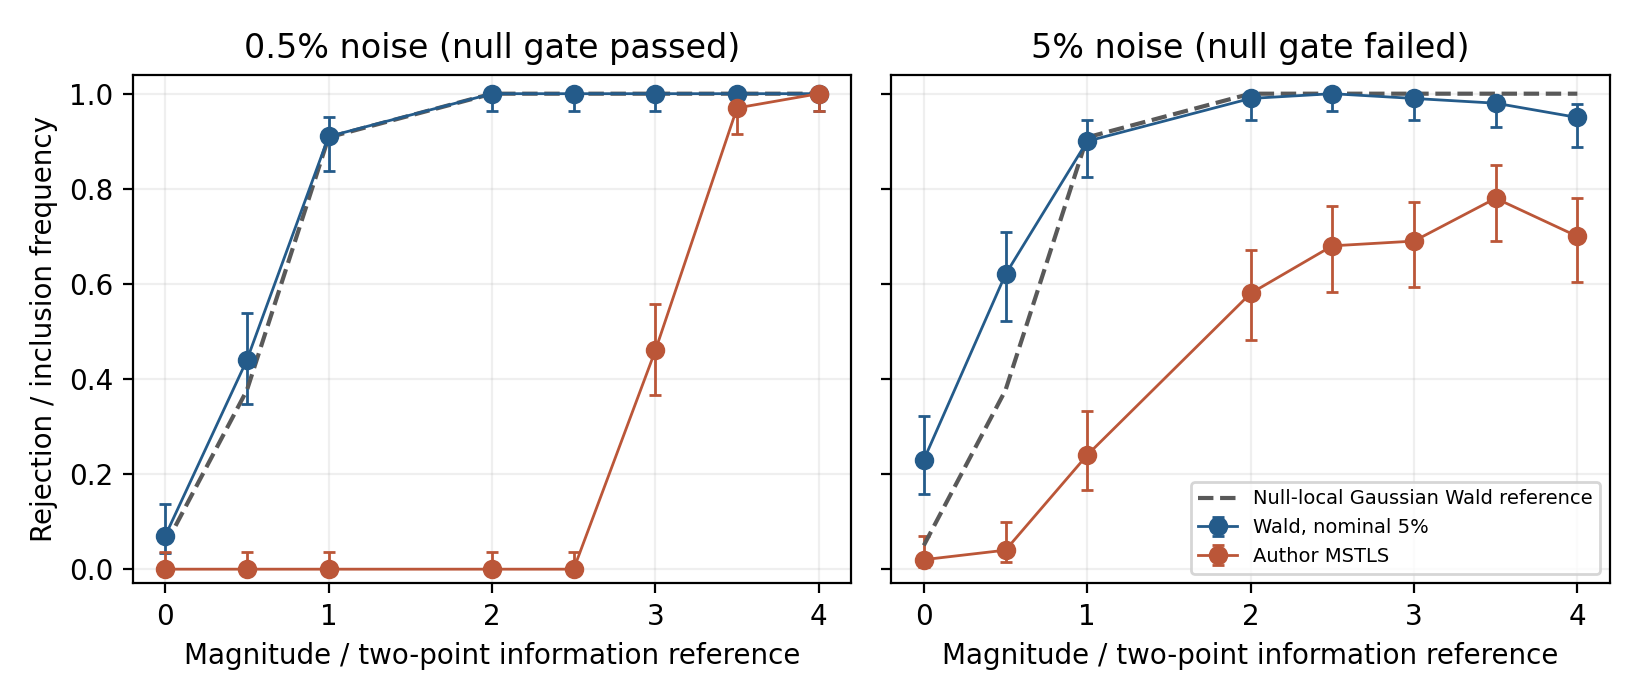
\includegraphics[keepaspectratio,alt={Figure S1. Paired rejection/inclusion frequencies for the added negative cubic term, with Wilson 95\% intervals and 100 paths per point. The dashed curve is the two-sided Gaussian Wald reference computed from null local efficient information; the horizontal scale uses a distinct equal-prior two-point error reference. At one unit its Wald prediction is about 90.8\%. The small-noise null-calibration gate passes; the 5\% gate fails, so the right-panel Wald frequencies are descriptive. Finite alternatives need not follow the null-local curve.}]{figures/publication/support_wald_mstls.png}}
\setcounter{figure}{0}
\caption{Paired rejection/inclusion frequencies for the added
negative cubic term, with Wilson 95\% intervals and 100 paths per point.
The dashed curve is the two-sided Gaussian Wald reference computed from
null local efficient information; the horizontal scale uses a distinct
equal-prior two-point error reference. At one unit its Wald prediction
is about 90.8\%. The small-noise null-calibration gate passes; the 5\%
gate fails, so the right-panel Wald frequencies are descriptive. Finite
alternatives need not follow the null-local curve.}
\end{figure}

\subsubsection{S3.2. Boundary-valid intervals for paired frequency
differences}\label{s3.2.-boundary-valid-intervals-for-paired-frequency-differences}

Let \(p_{10}=P(W=1,M=0)\) and \(p_{01}=P(W=0,M=1)\) for the targeted
Wald outcome \(W\) and MSTLS inclusion \(M\) on the same path. Their
frequency difference is \(\Delta=p_{10}-p_{01}\). For \(n\) independent
paths, the two discordant counts have binomial marginals; they are not
independent of each other. We construct two-sided Clopper--Pearson
intervals {[}4{]} \([L_{10},U_{10}]\) and \([L_{01},U_{01}]\), each with
confidence \(1-\alpha/2\). Bonferroni then gives simultaneous coverage
at least \(1-\alpha\) for these two probabilities, without assuming
independence. Projection yields the conservative pointwise interval

\[
\Delta\in[L_{10}-U_{01},\ U_{10}-L_{01}]\cap[-1,1].
\]

For \(\alpha=0.05\), each individual interval has confidence 97.5\% and
each tail probability is 0.0125. At \(n_{10}=100,n_{01}=0\) the result
is \([0.914252,1]\); at \(n_{10}=n_{01}=0\) it is
\([-0.042874,0.042874]\). Thus extreme samples retain uncertainty. These
intervals can be wider than paired score intervals {[}5{]}; we use the
conservative construction for an explicit finite-sample guarantee.
Coverage is pointwise for each grid cell, not simultaneous across the
whole alternative grid.

This is a post-study correction of uncertainty reporting prompted by
degenerate percentile bootstrap intervals. All 1600 paired outcomes, the
rejection/inclusion counts, nominal thresholds and Wilson compatibility
gate are unchanged. The original bootstrap results remain archived;
\texttt{reports/support\_wald\_paired\_intervals.json} stores both
versions and all four joint-cell counts. The local one-unit difference
remains 91 percentage points, now with interval 78.2--96.3 points. It
compares different operating outcomes, not tests with common size or
general structure-selection accuracy.

\subsection{S4. Same-path null calibration with random-design and
bootstrap
SEs}\label{s4.-same-path-null-calibration-with-random-design-and-bootstrap-ses}

The configuration \texttt{configs/wald\_se\_calibration.json} was frozen
before any new SE outcomes;
\texttt{reports/wald\_se\_protocol\_decision.json} records its timestamp
and SHA256 together with the archived-reference hash. All 100 previously
evaluated null paths at 5\% noise are retained. Five shards contain
twenty paths each, assigned by seed modulo five. Their observed input
hashes, all eighteen coefficients and nominal standard errors are
replayed against the archived reference. The point estimates and
\(z_{0.975}\) cutoff are common to the three SE branches. No
outcome-dependent SE scaling, bias correction or empirical rejection
cutoff is introduced. These known null paths provide a paired diagnostic
rather than independent confirmation.

\subsubsection{S4.1. Random-design score
sandwich}\label{s4.1.-random-design-score-sandwich}

Let \(m(\theta)=b-A\theta\), with Hermite-corrected \(A\), and fix the
observed weights \(W=(C+\lambda I)^{-1}\) using the original relative
ridge rule. The observed bread is \(H=A^\top WA\). Generate OU
observations from a null-imposed bounded core-five pilot trajectory
\(x_0\) with coefficient vector \(\theta_0\) in the eighteen-dimensional
library. Four fitted background coefficients are retained and the
candidate is set to zero; the initial state and stationary OU covariance
are supplied. Subtract the clean generating trajectory's deterministic
discrete residual \(d_0=b(x_0)-A(x_0)\theta_0\). For each model draw,
form

\[
\psi^*=e_j^\top H^{-1}(A^*)^\top W\{b^*-d_0-A^*\theta_0\}.
\]

Here \(e_j\) selects the candidate at zero-based library index 14. The
SE is the centered sample standard deviation of 999 independent
\(\psi^*\) draws. Random \(A^*\) shares the observation noise with
\(b^*\), so the score variance includes their dependence and polynomial
design noise. This is Monte Carlo estimation of a model score
covariance, with fixed observed weights and bread. It leaves
pilot-weight variability to the full-refit bootstrap branch and leaves
score centering errors uncorrected. The recorded average score influence
across observed paths is 0.03462; its nonzero value cautions against
interpreting the sandwich as an exact finite-noise variance identity.
With deterministic \(A\), the influence projection reduces algebraically
to the fixed-weight GLS map.

\subsubsection{S4.2. Full-refit parametric
bootstrap}\label{s4.2.-full-refit-parametric-bootstrap}

For each observed path, 399 stationary OU draws are generated around the
same null-imposed pilot trajectory, with the original coordinate noise
scales. Each draw refits the thirty-window bounded core-five pilot,
integrates its fitted trajectory, rebuilds exact Hermite residual
covariance and the pilot quadrature correction, and fits all eighteen
coefficients on the original 480 windows. The SE is the target's sample
standard deviation with denominator \(B-1\). It measures variability of
this complete fitted procedure under the supplied pilot model. The mean
bootstrap target averaged across paths is \(-0.006910\); bootstrap bias
is recorded but not subtracted from observed estimates.

Bootstrap seeds are \(95000000+1000s+b\) and score seeds are
\(96000000+1000s+b\), for observed seed \(s\) and zero-based draw \(b\).
They occupy disjoint ranges and differ from the observation seeds. The
generating pilot restriction and supplied covariance remain substantive
assumptions. Any failed integration or fit stops its shard; replicates
are never silently removed. A separate one-path numerical smoke with
eight score draws and four bootstrap refits validates execution and
replay only.

\subsubsection{S4.3. Complete outcomes and
audit}\label{s4.3.-complete-outcomes-and-audit}

\begin{center}
\begin{minipage}{\linewidth}
Table S2. Null rejection on 100 paired Van der Pol paths at 5\% noise.
The frozen gate is inclusion of 5\% in the Wilson 95\% interval. The SE
ratio is the median of pathwise ratios to the nominal SE. The paths were
previously examined; this is a diagnostic, with independent confirmation
outstanding.

\small\setlength{\tabcolsep}{3pt}
\begin{tabular}{@{}lrllr@{}}
\toprule\noalign{}
Standard error & Rejections & Wilson 95\% & Gate & Median SE ratio \\
\midrule\noalign{}
Nominal & 23/100 & 15.8--32.2\% & Fail & 1.00 \\
Random-design sandwich & 2/100 & 0.6--7.0\% & Pass & 2.81 \\
Full-refit parametric bootstrap & 5/100 & 2.2--11.2\% & Pass & 1.79 \\
\bottomrule
\end{tabular}
\end{minipage}
\end{center}

Table S2 reports the full diagnostic: nominal 23/100 (Wilson
15.8--32.2\%), random-design sandwich 2/100 (0.6--7.0\%), and full-refit
bootstrap 5/100 (2.2--11.2\%). Both revised intervals include 5\%,
satisfying the frozen criterion. Median SEs are 0.04325, 0.12575 and
0.07862 respectively. Median paired ratios are 1, 2.812 and 1.792;
ratios of marginal medians are a different statistic. All original
target estimates and nominal SEs replay with zero numerical difference.
All 39,900 bootstrap targets are retained, their sample SDs are
recomputed, and all 300 rejection decisions are checked against the
unchanged normal cutoff. All 99,900 score draws were completed. Shard
runtimes range from 3.75 to 5.07 hours; aggregate bootstrap and score
times are 23.23 and 0.522 aggregate hours.

The byte-preserved outputs and execution logs are in
\texttt{data/wald\_se\_calibration/}, with a SHA256 inventory and
per-stage frozen-source audits.
\texttt{python\ scripts/finish\_wald\_se\_calibration.py\ -\/-analyze-only}
verifies that inventory and regenerates results from the committed
bundle without Kaggle access or ODE solves. No alternative-power samples
use the new SEs. Wilson compatibility on the previously examined 100
null paths motivates independent confirmation, rather than establishing
precise size, efficiency or post-selection validity.

\subsection{S5. Additional numerical checks and detailed
protocols}\label{s5.-additional-numerical-checks-and-detailed-protocols}

These checks preserve the supplementary numerical evidence and
implementation details of the condensed main paper. They use the
original archived data without new simulations or amended outcomes.

\subsubsection{S5.1. Scalar optimal-test
check}\label{s5.1.-scalar-optimal-test-check}

The scalar model is \(x'=ax\), with \(a=-1\), \(x_0=2\), \(T=4\) and OU
correlation time 0.4. Noise standard deviations are 0.1, 0.02 and 0.005.
For each amplitude, 1000 independent OU paths are shared across tests. A
30-window weak OLS pilot, clipped to \([-2.5,0.5]\), is substituted into
the explicit function of Section 5.3. A quintic cutoff is zero within a
quarter of the declared width from either endpoint and reaches one at
that width. Widths are 0.2, 0.1, 0.05, 0.025 and 0.0125. Simpson
quadrature uses \(h=1/16384\). The generating-parameter test is an
oracle comparison; the fitted-pilot test receives no true coefficient.

Unguarded weak ratios can have infinite population moments (Section
4.2). Reported scalar RMSE therefore uses the prespecified clipping of
final estimates to \([-2.5,0.5]\); unbounded medians are also archived.
The clean-moment denominator is reported solely as a diagnostic; every
path is retained. Only five final estimates are clipped, all from the
one-window comparator at noise SD 0.1; no oracle or fitted-optimal-test
estimate is clipped. Every path enters the summaries. Full counts are
listed in research archive S8.

\begin{center}
\begin{minipage}{\linewidth}
Table S3. Scalar coefficient errors at cutoff width 0.0125, with 1000
paired paths per amplitude. Medians are absolute errors; RMSE uses
bounded final estimates. The reference is the standard deviation of the
efficient Gaussian influence, for local information comparison.

\small\setlength{\tabcolsep}{3pt}
\begin{tabular}{@{}
  >{\raggedright\arraybackslash}p{(\linewidth - 8\tabcolsep) * \real{0.1579}}
  >{\raggedleft\arraybackslash}p{(\linewidth - 8\tabcolsep) * \real{0.2105}}
  >{\raggedleft\arraybackslash}p{(\linewidth - 8\tabcolsep) * \real{0.2105}}
  >{\raggedleft\arraybackslash}p{(\linewidth - 8\tabcolsep) * \real{0.2105}}
  >{\raggedleft\arraybackslash}p{(\linewidth - 8\tabcolsep) * \real{0.2105}}@{}}
\toprule\noalign{}
\begin{minipage}[b]{\linewidth}\raggedright
Noise SD
\end{minipage} & \begin{minipage}[b]{\linewidth}\raggedleft
One-window median
\end{minipage} & \begin{minipage}[b]{\linewidth}\raggedleft
Pilot-test median (95\% interval)
\end{minipage} & \begin{minipage}[b]{\linewidth}\raggedleft
Pilot-test RMSE
\end{minipage} & \begin{minipage}[b]{\linewidth}\raggedleft
Weak influence SD
\end{minipage} \\
\midrule\noalign{}
0.1 & 0.22443 & 0.05981 {[}0.05662, 0.06437{]} & 0.09035 & 0.09063 \\
0.02 & 0.04585 & 0.01248 {[}0.01159, 0.01331{]} & 0.01818 & 0.01813 \\
0.005 & 0.01141 & 0.00312 {[}0.00289, 0.00336{]} & 0.00455 & 0.00453 \\
\bottomrule
\end{tabular}
\end{minipage}
\end{center}

At noise SD 0.1, the fitted-pilot median is 0.05981, compared with
0.22443 for the fixed window. The Gaussian absolute-error median at the
class bound is 0.06113. These are different statistical summaries;
covariance efficiency is assessed separately by linearized variance. At
the smallest noise the pilot-test bias is 0.000050 and dispersion
0.004551. The oracle local efficiency relative to the weak-class bound
at width 0.0125 is 0.9864. Full width and amplitude dependence is
retained in research archive S8.

\begin{figure}[p]
\centering
\pandocbounded{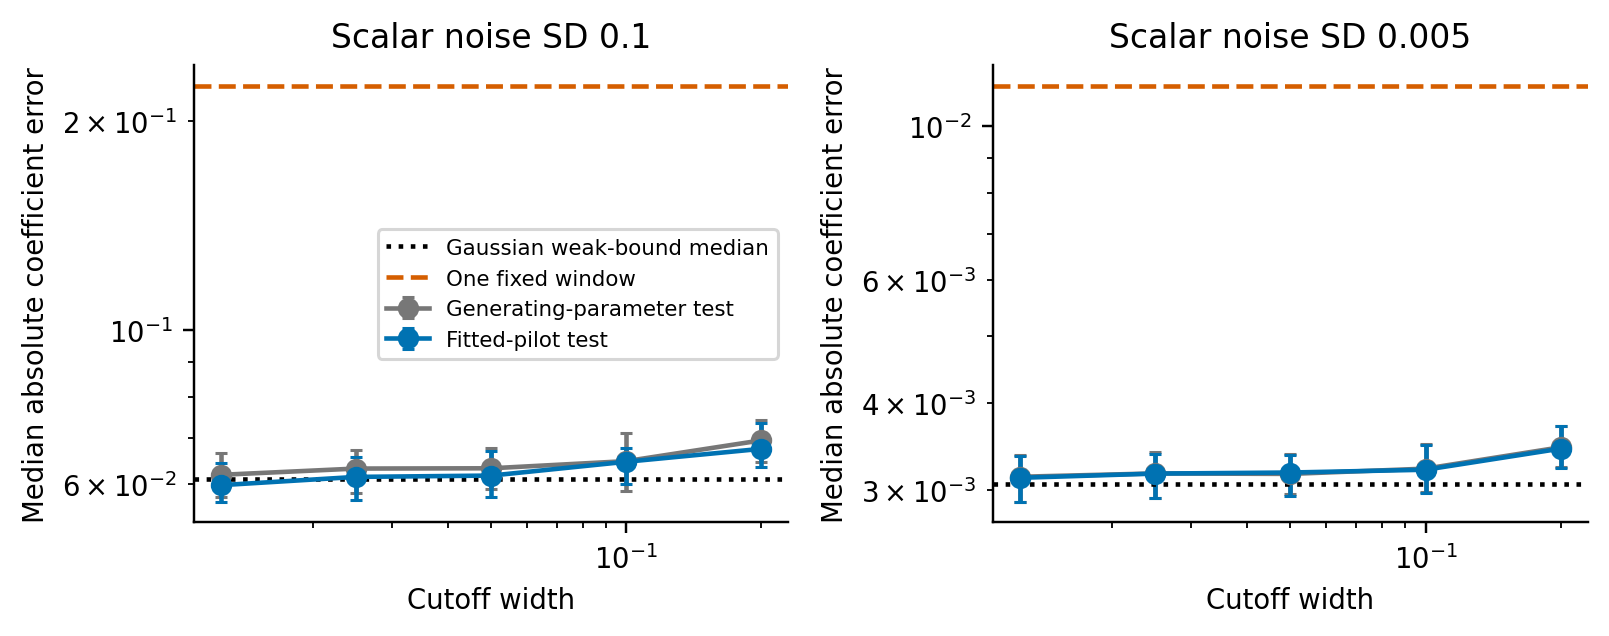
\includegraphics[keepaspectratio,alt={Figure S2. Scalar compact optimal tests at two noise amplitudes. Intervals resample independent paths; the dotted Gaussian median reference is derived from the sharp influence bound.}]{figures/publication/efficient_scalar.png}}
\setcounter{figure}{1}
\caption{Scalar compact optimal tests at two noise
amplitudes. Intervals resample independent paths; the dotted Gaussian
median reference is derived from the sharp influence bound.}
\end{figure}

\subsubsection{S5.2. Original 128-path nested-span
check}\label{s5.2.-original-128-path-nested-span-check}

The largest clean discrete GLS coefficient error is 2.82e-07, below the
small-noise error scale. For the feasible test, 128 independent paths at
each amplitude are shared by both weights and all three families.
Hermite-corrected moments use known marginal variances. A 30-window OLS
pilot is clipped to a fixed physical parameter box and integrated from
the known initial state. Exact polynomial covariance is evaluated on
this fitted model trajectory, and coefficient-dependent weights are
updated for at most 100 iterations, with relative tolerance \(10^{-7}\).
The covariance uses the fitted trajectory. This is a known-support
WENDy-like component; the complete author WENDy benchmark is documented
separately in research archive S6 and research archive S9.6.

\begin{center}
\begin{minipage}{\linewidth}
Table S4. Feasible Van der Pol empirical relative RMSE and 95\% path
bootstrap intervals, with 128 paired paths per row. Bias and dispersion
refer to the OU-weighted coefficient errors; their squares sum to
empirical MSE. Final coefficient estimates are unbounded; Proposition 3
concerns a distinct guarded routine and supplies no population-moment
guarantee for these archived fits.

\small\setlength{\tabcolsep}{3pt}
\begin{tabular}{@{}
  >{\raggedright\arraybackslash}p{(\linewidth - 10\tabcolsep) * \real{0.1304}}
  >{\raggedleft\arraybackslash}p{(\linewidth - 10\tabcolsep) * \real{0.1739}}
  >{\raggedleft\arraybackslash}p{(\linewidth - 10\tabcolsep) * \real{0.1739}}
  >{\raggedleft\arraybackslash}p{(\linewidth - 10\tabcolsep) * \real{0.1739}}
  >{\raggedleft\arraybackslash}p{(\linewidth - 10\tabcolsep) * \real{0.1739}}
  >{\raggedleft\arraybackslash}p{(\linewidth - 10\tabcolsep) * \real{0.1739}}@{}}
\toprule\noalign{}
\begin{minipage}[b]{\linewidth}\raggedright
Noise
\end{minipage} & \begin{minipage}[b]{\linewidth}\raggedleft
Windows
\end{minipage} & \begin{minipage}[b]{\linewidth}\raggedleft
OU RMSE (95\% interval)
\end{minipage} & \begin{minipage}[b]{\linewidth}\raggedleft
iid RMSE (95\% interval)
\end{minipage} & \begin{minipage}[b]{\linewidth}\raggedleft
OU bias
\end{minipage} & \begin{minipage}[b]{\linewidth}\raggedleft
OU dispersion
\end{minipage} \\
\midrule\noalign{}
0.5\% & 30 & 0.00200 {[}0.00181, 0.00220{]} & 0.00203 {[}0.00184,
0.00223{]} & 0.00027 & 0.00198 \\
0.5\% & 120 & 0.00173 {[}0.00156, 0.00190{]} & 0.00177 {[}0.00161,
0.00194{]} & 0.00010 & 0.00173 \\
0.5\% & 480 & 0.00174 {[}0.00157, 0.00190{]} & 0.00178 {[}0.00161,
0.00194{]} & 0.00011 & 0.00173 \\
5\% & 30 & 0.02711 {[}0.02437, 0.02993{]} & 0.02744 {[}0.02439,
0.03050{]} & 0.00900 & 0.02557 \\
5\% & 120 & 0.02545 {[}0.02277, 0.02810{]} & 0.02548 {[}0.02286,
0.02819{]} & 0.00770 & 0.02426 \\
5\% & 480 & 0.02558 {[}0.02288, 0.02833{]} & 0.02551 {[}0.02295,
0.02799{]} & 0.00814 & 0.02425 \\
\bottomrule
\end{tabular}
\end{minipage}
\end{center}

At 0.5\% noise, OU weighting with 480 windows gives empirical RMSE
0.001737, versus the sharp reference 0.001690. At 5\% noise it gives
0.025583, versus 0.016904; bias 0.008143 and dispersion 0.024253
identify finite-noise excess error. The stronger finite-noise assertion
that more windows alone would reach 0.016904 is therefore not supported
by this feasible implementation. The small-noise result and
deterministic geometry support the conditional efficiency mechanism,
while the moderate-noise result delimits it.

At 0.5\% noise, paired iid-minus-OU RMSE for 480 windows is 0.000038,
with 95\% interval {[}-0.000038, 0.000116{]}. At 5\% noise, paired
iid-minus-OU RMSE for 480 windows is -0.000075, with 95\% interval
{[}-0.001295, 0.001045{]}. These original 128-path intervals include
zero. The planned 2000-path follow-up in Section 7.1 resolves the
small-noise weighting comparison. Intervals are pointwise across
comparisons. All 1536 final fits meet the stopping tolerance within 23
iterations, and no pilot is clipped; the finite-noise gap persists after
this convergence control. Stopping counts are retained in research
archive S8; no path is excluded.

\begin{figure}[p]
\centering
\pandocbounded{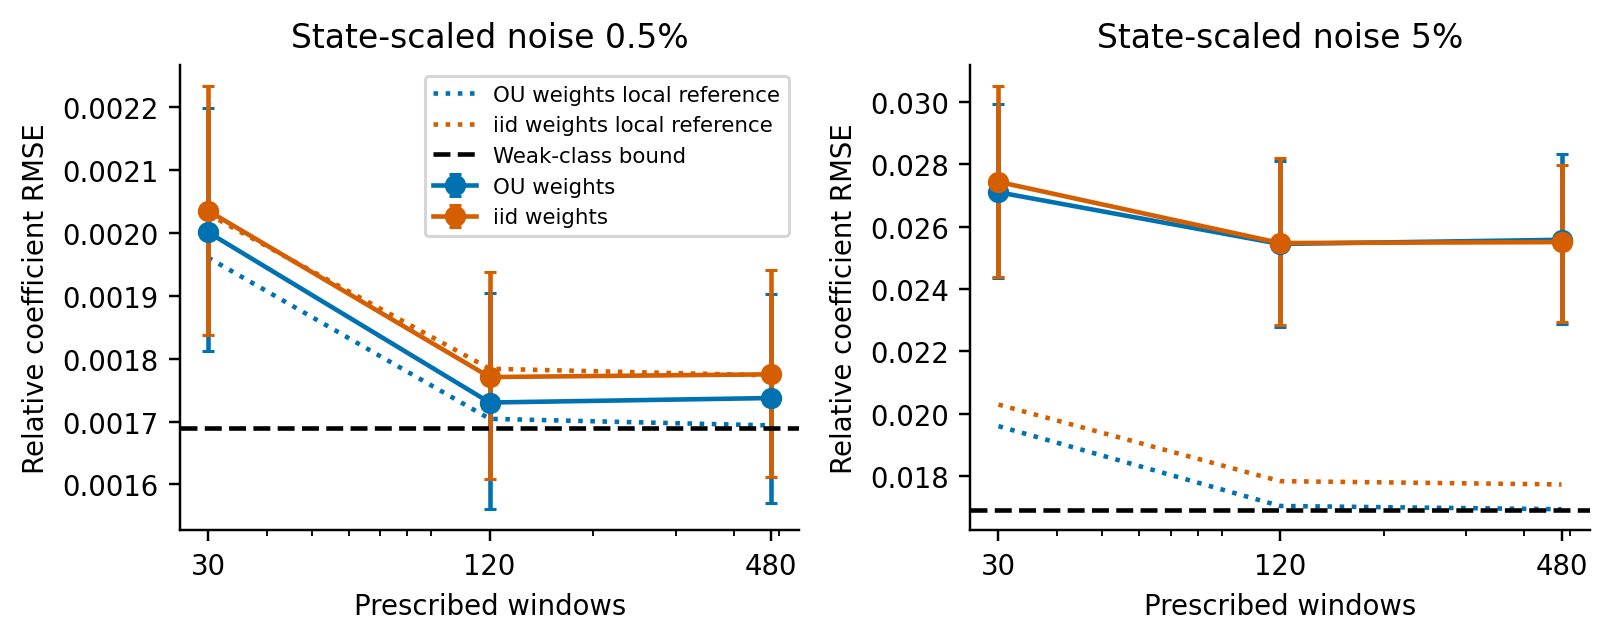
\includegraphics[keepaspectratio,alt={Figure S3. Feasible Van der Pol RMSE as the test span grows. Dotted curves show oracle local influences and the horizontal dashed line the class reference. At 0.5\% noise the dotted iid local reference nearly overlaps the empirical iid curve. Each empirical point uses the original 128 paired paths; the 2000-path 480-window comparison is reported separately.}]{figures/publication/efficient_vdp.png}}
\setcounter{figure}{2}
\caption{Feasible Van der Pol RMSE as the test span grows.
Dotted curves show oracle local influences and the horizontal dashed
line the class reference. At 0.5\% noise the dotted iid local reference
nearly overlaps the empirical iid curve. Each empirical point uses the
original 128 paired paths; the 2000-path 480-window comparison is
reported separately.}
\end{figure}

\subsubsection{S5.3. Matched author WENDy and moderate-noise
likelihood}\label{s5.3.-matched-author-wendy-and-moderate-noise-likelihood}

The pinned author WENDy implementation, including its own noise
estimation, test-radius selection, basis construction and stopping rule,
is run on exactly the 128 observations used by the feasible weak-GLS
experiment at \(h=0.005\). The supplied support has the same four free
coefficients. This isolates the observation protocol while allowing each
pipeline its declared estimator design. The same planned 128 seeds were
partitioned across four CPU jobs for throughput; each seed enters the
analysis once.

\begin{center}
\begin{minipage}{\linewidth}
Table S5. Matched Van der Pol comparison at 5\% noise, 128 paired paths.
Bootstrap intervals resample common seed indices. Bias and dispersion
use all coefficient vectors.

\small\setlength{\tabcolsep}{3pt}
\begin{tabular}{@{}
  >{\raggedright\arraybackslash}p{(\linewidth - 6\tabcolsep) * \real{0.2000}}
  >{\raggedleft\arraybackslash}p{(\linewidth - 6\tabcolsep) * \real{0.2667}}
  >{\raggedleft\arraybackslash}p{(\linewidth - 6\tabcolsep) * \real{0.2667}}
  >{\raggedleft\arraybackslash}p{(\linewidth - 6\tabcolsep) * \real{0.2667}}@{}}
\toprule\noalign{}
\begin{minipage}[b]{\linewidth}\raggedright
Estimator
\end{minipage} & \begin{minipage}[b]{\linewidth}\raggedleft
RMSE (95\% interval)
\end{minipage} & \begin{minipage}[b]{\linewidth}\raggedleft
Bias
\end{minipage} & \begin{minipage}[b]{\linewidth}\raggedleft
Dispersion
\end{minipage} \\
\midrule\noalign{}
Author WENDy & 0.024054 {[}0.021949, 0.026181{]} & 0.008557 &
0.022481 \\
OU weak GLS, 480 & 0.025583 {[}0.022840, 0.028227{]} & 0.008143 &
0.024253 \\
iid weak GLS, 480 & 0.025509 {[}0.022987, 0.028270{]} & 0.008464 &
0.024063 \\
\bottomrule
\end{tabular}
\end{minipage}
\end{center}

The paired OU-GLS-minus-author RMSE difference is 0.001529, with
interval {[}-0.000796, 0.004051{]}. The author pipeline has a 6.0\%
lower point RMSE in this cohort, but the paired interval contains zero,
leaving the ordering unresolved. Both estimators retain bias of roughly
0.008 in relative coefficient norm; dispersion supplies most of their
squared error. The separate complete-pipeline benchmark in research
archive S9.6 uses 16 paths, different seeds and \(h=0.01\); its WENDy
RMSE 0.02154 and WmSINDy RMSE 0.01926 cannot be ranked against the
present 128-path result. At 5\% noise nonlinear residual and
random-design terms, pilot error and estimator bias remain relevant
(research archive S3 and research archive S9.3). Their effects remain
under exact residual covariance. Adaptive radii and estimator-specific
bias handling are possible differences, but no ablation attributes the
gap to them. Small-noise efficiency is therefore not a claim of superior
practical accuracy at 5\%. Full WmSINDy also uses predictive and
noise-reconstruction losses; its estimating equation is not restricted
to the boundary-free class, so 0.016904 is not asserted as a lower bound
for it.

A separate bounded local Gaussian path-likelihood optimization at 5\%
uses these identical 128 observations and exact stationary OU
innovations. With the initial state known, relative RMSE is 0.01421
(95\% path-bootstrap interval {[}0.01290, 0.01549{]}); jointly fitting
its two coordinates gives 0.01720 ({[}0.01556, 0.01883{]}). Analytical
ODE sensitivities supply the Jacobian. All fits meet the optimizer's
stopping conditions, and 0 activate a declared parameter bound. These
local likelihood references quantify full-path accuracy at moderate
noise separately from the weak component (research archive S19).

On these same 128 records at 5\% noise, unknown-initial local likelihood
has RMSE 0.0172, author WENDy 0.0241 and weak GLS 0.0256. The weak
estimates have approximately 40\% and 49\% higher RMSE than likelihood,
respectively. This finite-noise comparison lies within the same
nuisance-initial-state information class; local small-noise efficiency
alone does not predict the moderate-noise ordering.

\subsubsection{S5.4. Sensitivity to supplied and fitted OU
shape}\label{s5.4.-sensitivity-to-supplied-and-fitted-ou-shape}

A separate 128-path Van der Pol check changes temporal weights to
\(\tau/2\) and \(2\tau\), keeping the correction variance known. At
0.5\% noise the RMSEs are 0.001747 and 0.001794, versus 0.001737 with
the correct shape; at 5\% they are 0.026242 and 0.026158, versus
0.025583. A stationary OU residual-profile fit using one known-initial
scoring step gives RMSE 0.0017366 and 0.025183 at the two amplitudes.
This check assesses a feasible residual plug-in; all fits converge
(research archive S12). Fixed-horizon infill identifies the microergodic
combination \(\sigma_j^2/\tau\), while separate variance and range
consistency requires additional acquisition or calibration {[}3, 6{]}.

\subsubsection{S5.5. Detailed protocols for the retained
comparisons}\label{s5.5.-detailed-protocols-for-the-retained-comparisons}

\textbf{Small-noise weighting and full-path likelihood references}

The follow-up uses 2000 prespecified seeds, including the original
128-path prefix exactly once. Its coefficients reproduce that prefix
without numerical discrepancy. All methods share the same observations
at 0.5\% noise. OU and iid weak GLS retain 480 prescribed windows (479
independent tests). The path-likelihood reference uses exact stationary
OU innovations and ODE sensitivities, starting from the feasible OU weak
estimate. One Fisher-scoring step holds the known initial state fixed,
or jointly updates four coefficients and two initial coordinates from
the noisy first observation. It is a local likelihood refinement. The
follow-up was planned after inspecting the original 128-path comparison;
5000 paired bootstrap draws quantify Monte Carlo uncertainty without
sequential stopping.

OU minus iid weighting is assessed by the paired iid-minus-OU RMSE
difference 0.00007426, with 95\% interval {[}0.00005576, 0.00009327{]}.
OU weighting reduces empirical RMSE by 4.22\%. On the additional 1872
paths alone, the interval also excludes zero. The main improvement comes
from enriching the test span; correct temporal covariance adds a
smaller, roughly 4--5\% improvement. OU weak RMSE 0.001685 is consistent
with the sharp reference 0.001690, within the local reference
uncertainty.

The known-initial one-step reference agrees with its information scale.
The unknown-initial one-step estimate retains bias 0.000469:
initialization at a noisy endpoint leaves appreciable nonlinear
remainder at this amplitude. After inspecting that result, two
additional scoring steps were computed on the same 2000 observations,
giving RMSE 0.001669 and bias 0.000068. This refinement is reported as a
likelihood-refinement follow-up on the same observations. The theorem
concerns the limiting influence; the scoring implementation also needs a
sufficiently accurate local initialization. The information lost when
the initial state is known is the projection
\(\mathcal I_{\theta u}\mathcal I_{uu}^{-1}\mathcal I_{u\theta}\); when
it is unknown, weak influences incur no further first-order loss
relative to the nuisance-adjusted path likelihood.

\textbf{Known-initial information recovery with universal endpoint
tests}

For known \(u\), extend the corrected residual to tests with nonzero
endpoint traces:

\[
m_\phi(\theta)=-\int_0^T[\phi'(t)^TY(t)+\phi(t)^Tf_\theta^H(Y(t))]dt
+\phi(T)^TY(T)-\phi(0)^Tu.
\]

Here \(f_\theta^H\) denotes coordinatewise Hermite correction under the
supplied sensor variance. Theorem 2 gives the full closed influence
class when \(u\) is known.

We compare four branches on 1968 identical records, indices 33--2000 of
the 0.5\% OU-noise study. Model-adjoint tests, integrated at each
record's pilot, are combined with the two controls \(Y(0)-u\). Their
span contains the efficient score directions in first order; agreement
with likelihood therefore checks this realization. The primary
alternative uses universal time-only tests: the original 480 interior
bumps plus twelve endpoint half-bumps of full widths 3, 1.5, 0.75,
0.375, 0.1875 and 0.09375, centered at 0 and 20, together with the same
initial controls. Joint \(H^1\) orthogonalization retains 491 scalar
tests. Exact discretized Hermite covariance includes all endpoint cross
terms. Composite Simpson integration gives clean-mean coefficient error
\(9.68\times10^{-7}\), below the frozen \(1.4\times10^{-5}\) gate. The
covariance weights still use a directly integrated pilot model; only
construction of the universal windows is independent of the ODE.

Before evaluating these endpoint branches, we replaced an absolute
screen threshold by two paired relative criteria: model-adjoint RMSE at
most 1.05 times the known-initial likelihood reference, and universal
tests closing at least 50\% of the original weak-to-likelihood RMSE gap.
The original absolute threshold failed even for likelihood on the
32-record screen and was unsuitable for that comparison. The amendment
and unchanged earlier outcomes are archived. The 1968 records were
unused for endpoint fitting; their original weak and likelihood outcomes
were already archived, so this is endpoint holdout confirmation rather
than an entirely unseen dataset. The likelihood reference is one
Fisher-scoring step with known \(u\), as in Section 7.1.

Universal endpoint tests close 97.1\% of the paired RMSE gap, with a
95\% paired-bootstrap interval of 95.5--98.6\%; their RMSE is 0.88\%
above the scoring reference. The model-adjoint/scoring ratio is 0.99954,
with interval 0.99815--1.00086. Both frozen point criteria are
satisfied. Bootstrap intervals use 5000 shared record resamples. Median
online times, including the common 30-window pilot, are 1.51 s for the
universal branch and 1.25 s for the model-adjoint branch; archived
scoring times were unavailable. The result establishes recovery by this
universal test family at small noise. Its model-based covariance pilot
prevents interpreting it as a fully ODE-free estimator or a demonstrated
computational advantage.

\textbf{Endpoint-component attribution}

The frozen ablation uses the same 500 records (indices 33--532). It is
component attribution on already evaluated data. All new branches use
identical Simpson quadrature and the same covariance-pilot rule; a
matched boundary-free branch isolates quadrature from endpoint changes.
The full branch and known-initial scoring are archived paired
references. For a positive matched baseline-to-scoring gap, the
prespecified material-contribution criterion is at least 50\% gap
recovery, with uncertainty reported separately.

Initial traces alone recover essentially the entire finite-family gap.
This is the mechanism already proposed by Brunel et al. {[}7{]}, with
its OU efficiency quantified here. The initial-noise controls provide a
measurable standalone improvement, but fail the 50\%
material-contribution rule. The all-minus-initial RMSE difference is
\(7.46\times10^{-8}\), with paired interval
\([-7.18\times10^{-7},8.55\times10^{-7}]\), giving no resolved
improvement over initial traces. Terminal traces alone give no resolved
improvement, consistent with the unchanged closed class in Theorem 2.
Component gains overlap; their percentages are not additive. The
archived trapezoidal boundary-free RMSE is 0.00164343, so quadrature
accounts for only 0.16\% of the matched gap. All intervals use 5000
shared bootstrap resamples. Recovery percentages can exceed 100\%
through Monte Carlo variation; they are not clipped.

\textbf{Added-term detection and the nuisance-adjusted reference}

An additional \(\delta x^3\) term in the second Van der Pol equation
gives a bounded structural alternative for negative \(\delta\),
retaining the stabilizing \(-x^2v\) term. Let \(s_\delta\) be its
sensitivity and let \(S_{-\delta}\) collect the other coefficient
sensitivities. The local composite likelihood information is
\(\|s_\delta-\Pi_{S_{-\delta}}s_\delta\|_{\mathcal H}^2\); the
boundary-free reference additionally projects on \(Z\). The local
equal-prior two-point error reference
\(\Phi(-|\delta|\sqrt{\mathcal I^{\mathrm{eff}}_{\delta}}/2)=0.05\)
gives
\(|\delta|_{\min}=2\Phi^{-1}(0.95)/\sqrt{\mathcal I^{\mathrm{eff}}_{\delta}}\).
This profiles nuisance coefficients rather than treating them as known
through a raw diagonal information entry.

For the full degree-one-through-three polynomial library in both
equations, profiling the 17 other coefficients gives local references
0.01928 with known initial state and 0.01941 for the boundary-free class
at 0.5\% noise. At 5\%, these become 0.19279 and 0.19410. The small
difference is direction specific; it differs from the aggregate
coefficient-RMSE cost. The complete pinned author's adaptive WSINDy,
with unchanged selection settings, was evaluated on 100 paired noise
paths at each of five negative alternatives per amplitude. At magnitudes
0, 0.5, 1, 2 and 4 times the local weak reference, inclusion counts are
0, 0, 0, 0 and 100 at 0.5\% noise, and 2, 4, 24, 58 and 70 at 5\%. Full
Wilson intervals and the core-five-coefficient comparison appear in
research archive S20. The local Gaussian reference describes regular
composite-model information; sparse selection on a fixed background and
finite-amplitude alternatives are different experiments. In particular,
the large 5\% alternatives require nonlinear interpretation. The
author's selection curve supplies an algorithmic benchmark, rather than
an equality test of the information formula.

\textbf{Moderate-noise endpoint confirmation}

The 128-record 5\% Van der Pol check uses the same observations as the
previous moderate-noise benchmark, with supplied covariance and known
\(u\). Its primary likelihood comparator therefore fixes \(u\); the
unknown-initial likelihood result supplies context. All new weak
branches share Simpson quadrature, a 480-window interior family and the
same 30-window covariance pilot. The universal branch adds the frozen
endpoint half-windows and initial controls. Source fingerprints and all
paired observation hashes are verified.

The universal branch recovers 32.6\% of the matched
weak-to-known-initial-MLE RMSE gap, with paired 95\% interval
18.3--45.8\%. The frozen 50\% criterion fails. Thus near-complete
small-noise recovery does not extend to this moderate-noise feasible
estimator. The archived trapezoidal weak RMSE, 0.0255834, is close to
the matched Simpson value.

At the clean design and true coefficients, the first-order covariance
reference gives relative RMSE 0.0130935 for the universal span and
0.0169382 for the compact span. Retaining all Hermite orders changes
these fixed-clean-design references to 0.0136355 and 0.0170083. Full
residual covariance therefore raises the universal surrogate scale by
4.1\%, while actual universal dispersion is 0.0211247 and its bias norm
is 0.0056954. These quantities distinguish the restored local geometry
from finite-noise performance. The covariance-surrogate difference is
not an exact decomposition of estimator variance: random designs,
same-record pilots and nonlinear fitting remain in the empirical
estimate.

\textbf{Lorenz endpoint confirmation}

The three-state confirmation uses the supplied Lorenz structure, known
\(u=(1,1,1)\), 0.5\% OU noise and all 256 frozen paired records. The
universal family adds twelve time-only endpoint half-windows and three
initial controls to 480 interior windows. Its covariance weights use the
same bounded 30-window pilot as the matched compact branch. The
comparator is fully optimized known-initial likelihood with exact
discrete OU innovations and analytical sensitivities. All fits converge;
none is excluded. Both clean-mean quadrature errors pass the fixed gate
(S2).

Universal endpoints recover 95.5\% of the paired compact-to-likelihood
RMSE gap, with interval 92.8--98.0\%, satisfying the frozen 50\%
criterion. The first-order universal clean-design reference is
0.00020891 and its full-Hermite counterpart is 0.00020926; the matched
compact references are 0.00041358 and 0.00041363. The empirical endpoint
dispersion is close to this local geometry. Together with the Van der
Pol ablation, this supports small-noise recovery across two supplied
polynomial structures. It does not extend the 97.1\% Van der Pol
percentage to arbitrary systems or moderate noise.

\textbf{Prespecified Wald rejection versus sparse inclusion}

We refine the added-cubic grid with 2.5, 3 and 3.5 reference units and
compare the author's unchanged MSTLS with a two-sided Wald test of the
single prespecified \(x^3\) coefficient at nominal 5\%. All eighteen
library coefficients are fitted without penalization by feasible weak
GLS on 480 compact tests. Exact Hermite residual covariance is evaluated
at a bounded core-five pilot. Original paired observations and author
fits are reused, and intermediate grid points share their noise seeds.
S3 documents a pilot-model correction of deterministic quadrature
defects, fixed before inspecting the first version's noisy Wald
outcomes. No significance or selection thresholds were tuned.

At 0.5\% noise, null rejection is 7/100 (Wilson interval 3.4--13.7\%),
passing the prespecified compatibility gate for nominal 5\%. One
reference unit gives 91\% rejection (83.8--95.2\%), consistent with the
90.8\% null-local Gaussian Wald prediction. MSTLS includes no target at
that magnitude and reaches 46\% at three units and 97\% at 3.5 units.
The paired one-unit difference is 91 percentage points, with
conservative paired interval 78.2--96.3 points (S3.2). These
supplied-candidate frequencies are consistent with the local small-noise
reference; they require independent size and power confirmation. With
only 100 null paths, passing the gate establishes compatibility, rather
than precise size calibration or efficiency over a growing library.

At 5\% noise, null Wald rejection is 23/100 (15.8--32.2\%), failing the
gate. The target's empirical null RMSE is 0.07578, versus median
reported standard error 0.04325; these are diagnostic scales, not an
exact variance ratio. The nominal standard errors leave finite-noise
random-design and pilot effects insufficiently calibrated. Higher
alternative rejection therefore gives no calibrated-power advantage at
this amplitude. MSTLS null inclusion is 2/100 (0.6--7.0\%); it has no
nominal test size parameter. Both panels are retained without repair
based on their outcomes. The comparison separates prespecified
statistical testing from library-wide sparse selection and
post-selection inference.

\subsection{S6. Supplementary local-estimation
details}\label{s6.-supplementary-local-estimation-details}

These details specialize classical estimating-equation and
efficient-score arguments {[}8--10{]}. Continuous-record linear
estimation and its discrete approximation are established by Dette,
Konstantinou and Zhigljavsky {[}11{]}; the main paper restricts their
local regression geometry through the dynamical adjoint range.

\subsubsection{S6.1. Scalar path information and weak-ratio
diagnostics}\label{s6.1.-scalar-path-information-and-weak-ratio-diagnostics}

For \(x_a(t)=x_0e^{at}\) with known \(x_0\), \(s(t)=x_0te^{at}\) and

\[
\mathcal I_T(a)=\frac{\tau x_0^2}{2\sigma^2}
\int_0^Te^{2at}[1+(a+\tau^{-1})t]^2\,dt.
\]

On a uniform grid, exact innovations give

\[
\mathcal I_h(a)=\frac{s(0)^2}{\sigma^2}+
\frac{\sum_{n=1}^N[s(t_n)-\rho s(t_{n-1})]^2}{\sigma^2(1-\rho^2)}
\longrightarrow\mathcal I_T(a),\qquad\rho=e^{-h/\tau}.
\]

Nested grids give increasing information bounded by \(\mathcal I_T\).
The limit follows from a Riemann sum of squared sensitivity innovations.
Statistical saturation therefore concerns the full experiment.

For \(D_\phi=\int\phi x_a\ne0\), a scalar weak ratio has limit

\[
\widehat a_h=\frac{-\mathcal Q_h(\phi'Y)}{\mathcal Q_h(\phi Y)}
\longrightarrow a+\frac{N_\phi}{D_\phi+E_\phi},\qquad
N_\phi=\int(-\phi'-a\phi)\eta_C,\quad E_\phi=\int\phi\eta_C.
\]

OU path continuity gives almost sure convergence of the quadratures. The
weights \(\phi\) and \(-\phi'-a\phi\) are independent: dependence would
make a nonzero compactly supported function solve a homogeneous
first-order equation. The OU kernel is strictly positive on nonzero
weights, so \((N_\phi,E_\phi)\) is nondegenerate Gaussian. Positive
conditional variance of \(N_\phi\) given \(E_\phi\) and positive
denominator density at zero imply infinite absolute and squared error
moments of the unguarded ratio. Its empirical summaries should use
quantiles or explicit guards.

The influence \(\ell=(-\phi'-a\phi)/D_\phi\) has Gaussian variance

\[
V_\phi=\iint\ell(s)C(s,t)\ell(t)dsdt.
\]

Differentiating the weak identity gives \(\int\ell s=1\).
Cauchy--Schwarz in the covariance RKHS gives

\[
1\leq V_\phi\mathcal I_T(a),\qquad
\operatorname{Eff}_\phi=[\mathcal I_T(a)V_\phi]^{-1}\leq1.
\]

This efficiency concerns the Gaussian linearization.

\subsubsection{S6.2. Proof of the conditional dense-span
proposition}\label{s6.2.-proof-of-the-conditional-dense-span-proposition}

This auxiliary conditional statement separates estimator regularity from
projection geometry. Proposition 3 derives its fixed-family conclusions
from primitive conditions; the assumptions below serve only to state the
separate projection argument:

\begin{itemize}
\tightlist
\item
  (P1) For each fixed finite family, the corrected weak solution has
  expansion
  \(\widehat\theta_{K,\epsilon}-\theta=\epsilon P_K r_K+o_p(\epsilon)\),
  with \(r_K\) centered Gaussian of covariance \(\Sigma_K\), and
  full-column-rank \(D_K\).
\item
  (P2) Feasible pilots and covariance weights change
  \(P_K=(D_K^\top\Sigma_K^{-1}D_K)^{-1}D_K^\top\Sigma_K^{-1}\) by
  \(o_p(1)\). Deterministic quadrature error is \(o(\epsilon)\).
\item
  (P3) The squared norms of
  \(\epsilon^{-1}(\widehat\theta_{K,\epsilon}-\theta)\) are uniformly
  integrable. Distributional convergence alone does not imply covariance
  convergence. Stable local solves with bounded fallback and bad-event
  probability \(o(\epsilon^2)\) are one possible sufficient
  implementation.
\item
  (P4) The deterministic, nested influence spans are dense in
  \(\mathcal M\) in covariance norm, and \(\mathcal I_{e,C}\) is
  positive definite.
\end{itemize}

\textbf{Proof.} Under (P1) and (P2), Slutsky's lemma gives the centered
Gaussian limit with covariance
\(P_K\Sigma_KP_K^\top=(D_K^\top\Sigma_K^{-1}D_K)^{-1}=V_K\). To see the
moment conclusion, let
\(X_\epsilon=\epsilon^{-1}(\widehat\theta_{K,\epsilon}-\theta)\).
Assumption (P3) and the continuous-mapping theorem give convergence of
each first and second coordinate moment:
\(|X_iX_j|\leq\|X_\epsilon\|^2\) supplies the necessary uniform
integrability. Hence \(E X_\epsilon\to0\) and
\(\operatorname{Cov}(X_\epsilon)\to V_K\). No risk conclusion is drawn
for an unguarded ratio lacking (P3).

Let \(t_i=C^{-1}R_i\in\mathcal M\) be the efficient dual representers of
the coefficient sensitivities from the boundary-free theorem, and let
\(Q_K\) be covariance-orthogonal projection onto the finite influence
span. Because every test influence annihilates \(Z\), its pairing with
\(S_i\) equals its pairing with \(R_i\). The finite-family information
is therefore

\[
(D_K^\top\Sigma_K^{-1}D_K)_{ij}
=\langle Q_Kt_i,Q_Kt_j\rangle_C.
\]

By (P4), \(Q_Kt_i\to t_i\) in covariance norm. Cauchy--Schwarz then
gives entrywise convergence to
\(\langle t_i,t_j\rangle_C=(\mathcal I_{e,C})_{ij}\). The nested
projected information matrices increase in Loewner order, and positive
definiteness makes matrix inversion continuous at the limit.
Consequently \(V_K\to\mathcal I_{e,C}^{-1}\). These are two sequential
limits. A joint \(K,\epsilon\) limit requires uniform controls absent
from (P1)--(P4). The proof is a specialization of classical
estimating-equation linearization and efficient-score projection {[}8,
9, 10 and 25{]}. \(\square\)

\subsubsection{S6.3. Parameter-dependent weak
likelihood}\label{s6.3.-parameter-dependent-weak-likelihood}

The same leading map arises from a parameter-dependent Gaussian weak
likelihood of the form studied by WENDy-MLE {[}12{]}, provided the
covariance shape is correct and the local solution is regular. For fixed
dimension write \(r(\theta)=\epsilon r_1+o_p(\epsilon)\),
\(\partial_\theta r=-D+o_p(1)\) and
\(\Sigma_\epsilon(\theta)=\epsilon^2\Sigma_0(\theta)\), with smooth
positive definite \(\Sigma_0\). The objective
\(\log\det\Sigma_\epsilon+r^T\Sigma_\epsilon^{-1}r\) has
covariance-derivative and log-determinant score terms of order
\(O_p(1)\) in an \(O_p(\epsilon)\) neighborhood; its mean-residual score
is of order \(O_p(\epsilon^{-1})\). The local score equation therefore
gives

\[
\widehat\theta-\theta=\epsilon
(D^T\Sigma_0^{-1}D)^{-1}D^T\Sigma_0^{-1}r_1+o_p(\epsilon).
\]

Thus the log determinant and covariance derivatives distinguish
finite-noise weak likelihood from frozen GLS, while both share the
correct-covariance leading influence under these assumptions. This
connects Proposition 3 to a regular local weak-likelihood estimator; its
assumptions concern a regular local optimizer and consistent covariance
calibration.

\subsubsection{S6.4. Raw features and linear-time temporal covariance
application}\label{s6.4.-raw-features-and-linear-time-temporal-covariance-application}

For correction variance \(\widehat v\), define

\[
\bar f=\exp\left[\frac12\sum_j(v_j-\widehat v_j)\partial_j^2\right]f.
\]

The exponential terminates for polynomials. Using \(\bar f\) in \(c\)
gives covariance, while mean residual is
\(\int\phi_k[f_i(x)-\bar f_i(x)]dt\). Raw monomials use
\(\widehat v=0\). Mean bias and covariance are separate outputs.

On a uniform grid, collect weighted coefficients into an \(N\times Kd\)
matrix \(\mathsf B_\alpha\). Each term is
\(\alpha!v^\alpha \mathsf B_\alpha^TR_{q,h}\mathsf B_\alpha\), where
\((R_{q,h})_{nm}=\rho_q^{|n-m|}\) and \(\rho_q=e^{-qh/\tau}\). For a
computational vector \(w\),

\[
a_n=w_n+\rho_qa_{n-1},\qquad z_n=w_n+\rho_qz_{n+1},\qquad
R_{q,h}w=a+z-w,
\]

with zero exterior initialization. Each multi-index costs \(O(N(Kd)^2)\)
time and \(O(NKd+(Kd)^2)\) memory, avoiding an \(N\times N\) temporal
matrix. An independent fixed-variance nugget has additional
diagonal-in-time covariance; its linear weak contribution is \(O(h)\).
The exact mixed-noise formula is in the supplement.

\subsubsection{S6.5. Explicit scalar OU optimal
test}\label{s6.5.-explicit-scalar-ou-optimal-test}

For scalar exponential dynamics, \(z=e^{at}\), \(s=x_0te^{at}\),
\(k=\mathcal I_{au}/\mathcal I_{uu}\) and \(g=e^{at}(x_0t-k)\). Define

\[
A_0=\frac{(1-\tau^2a^2)x_0}{2\sigma^2\tau},\qquad
B_0=\frac{-(1-\tau^2a^2)k-2\tau^2ax_0}{2\sigma^2\tau},
\]

\[
q_0=\frac{-k-\tau(x_0-ak)}{2\sigma^2},\qquad
F_j(t)=\int_0^t s^je^{2as}ds.
\]

Then

\[
\phi_*(t)=-\frac{e^{-at}}{\mathcal I_e}
[q_0+A_0F_1(t)+B_0F_0(t)].
\]

For \(a\ne0\), \(F_0=\operatorname{expm1}(2at)/(2a)\) and
\(F_1=[e^{2at}(2at-1)+1]/(4a^2)\); their continuous limits at \(a=0\)
are \(t\) and \(t^2/2\). A pilot coefficient substitutes into this
expression before a compact cutoff is applied. The explicit multivariate
fundamental-matrix expression is an analytical identity whose numerical
inversion depends on conditioning; strongly contracting dynamics can
make that inversion ill-conditioned.

\subsection{S7. Archived regularization and a constructive guarded
variant}\label{s7.-archived-regularization-and-a-constructive-guarded-variant}

\subsubsection{S7.1. What the archived solver actually
approaches}\label{s7.1.-what-the-archived-solver-actually-approaches}

Write \(q=\dim(\widehat\Sigma_\epsilon)\) for the number of residual
moments, distinct from the library size. In
\texttt{src/weak\_efficiency.py}, \texttt{gls\_map} adds
\(\lambda_\epsilon I=\rho\,\operatorname{tr}(\widehat\Sigma_\epsilon)I/q\)
to the physical residual covariance, with fixed relative
\(\rho=10^{-10}\) in the primary protocols. If
\(\epsilon^{-2}\widehat\Sigma_\epsilon\to\Sigma_1>0\), its normalized
limit is

\[
W_\rho=\left[\Sigma_1+\rho\operatorname{tr}(\Sigma_1)I/q\right]^{-1}.
\]

Thus fixed relative ridge is not removed by small-noise scaling.
Whenever a regular local expansion exists, the corresponding leading map
and covariance are

\[
P_\rho=(D^\top W_\rho D)^{-1}D^\top W_\rho,\qquad
V_\rho=P_\rho\Sigma_1P_\rho^\top.
\]

For the ideal map \(P_0\), both maps satisfy \(P_\rho D=P_0D=I\) and

\[
V_\rho-V_0=(P_\rho-P_0)\Sigma_1(P_\rho-P_0)^\top\succeq0.
\]

Indeed, \(P_0\Sigma_1=V_0D^\top\) annihilates the cross terms because
\((P_\rho-P_0)D=0\). Equality holds only when the two maps coincide; a
small numerical ridge alone gives no theorem-level equality. Its impact
also depends on conditioning. The archived final fits are unbounded and
their bounded covariance pilots do not control inverse random-design
tails. Neither uniform integrability nor exact ideal-GLS efficiency of
these archived algorithms is claimed. Their finite mesh and fixed
spectral cutoff also differ from the sequential limit in Proposition 3.

\subsubsection{S7.2. A specified algorithm for which the fixed-family
assumptions
follow}\label{s7.2.-a-specified-algorithm-for-which-the-fixed-family-assumptions-follow}

The separate routine \texttt{src/guarded\_gls.py} specifies a bounded
vanishing-ridge variant. It retains fixed, deterministic test functions
and the known sensor covariance model. It divides physical residual
covariance by \(\epsilon^2\), uses relative ridge
\(\rho_\epsilon=\epsilon^2\), and rejects a numerical solve when
normalized covariance or column-scaled normal-matrix relative minimum
eigenvalues fall below \(10^{-8}\epsilon^2\). A rejected solve returns
the fixed coefficient-box midpoint. A successful solve is projected onto
that same compact box. These safeguards leave a regular local solution
unchanged asymptotically. This routine is a new analytically specified
variant; none of the reported Monte Carlo outcomes uses it.

\textbf{Proposition 3 (guarded fixed-family weak GLS; detailed
assumptions).} Consider a correctly specified polynomial vector field
linear in its \(p\) coefficients, known initial state and supplied
independent-coordinate OU covariance shape with a common correlation
time. Fix a finite deterministic family of boundary-free tests. Assume:

\begin{itemize}
\tightlist
\item
  (G1) The true coefficient lies inside the final compact box. Its clean
  trajectory and nearby pilot-model trajectories exist on \([0,T]\) and
  depend smoothly on the pilot coefficients on a common bounded region.
\item
  (G2) The clean corrected design \(D\) and the clean design of a fixed
  finite-window pilot both have full column rank. The pilot's declared
  structural family contains the truth. Clipping the pilot to a compact
  convex box containing the truth is allowed, including truth on its
  boundary.
\item
  (G3) The first-order residual covariance \(\Sigma_1\) of this finite
  family is positive definite after exact dependencies are removed. The
  model covariance is evaluated from the full Hermite formula at the
  pilot, with known marginal correction variances.
\item
  (G4) Deterministic quadrature weights have uniformly bounded total
  absolute mass for each test and converge to their continuum integrals.
  Their clean residual and pilot-design errors are \(o(\epsilon)\). Any
  subtracted pilot-model quadrature defect has value \(o(\epsilon)\) and
  derivative \(o(1)\) uniformly near the truth. Tests and their first
  derivatives are bounded and have the required quadrature regularity.
\end{itemize}

Build the pilot by corrected least squares on its stated family, using a
fixed bounded fallback if its design is singular. Construct the full
Hermite covariance at the integrated pilot, and apply the guarded
routine above to the final corrected moments. Then, for fixed family
size,

\[
\epsilon^{-1}(\widehat\theta_\epsilon^{\mathrm{guard}}-\theta)
\Rightarrow N(0,V_K),\qquad
\epsilon^{-2}\operatorname{Cov}(\widehat\theta_\epsilon^{\mathrm{guard}})
\longrightarrow V_K=(D^\top\Sigma_1^{-1}D)^{-1}.
\]

The squared scaled errors are uniformly integrable. If this construction
is applied to nested dense admissible families satisfying (G1)--(G4)
separately, the subsequent family limit gives the boundary-free
covariance reference of Theorem 1. This is a sequential result; it
supplies no uniform rate in family size and no conclusion for an
unchanged fixed mesh or ridge.

\textbf{Proof.} Write \(Y=x+\epsilon\eta\) and \(M=\|\eta\|_\infty\).
For each OU coordinate,

\[
\eta_j(t)=e^{-t/\tau_j}
\left[\eta_j(0)+\sqrt{2\sigma_{0,j}^2/\tau_j}
\int_0^t e^{s/\tau_j}dW_j(s)\right].
\]

The stochastic integral is a martingale with a Gaussian terminal value
of finite variance. Doob's \(L^q\) inequality for \(q>1\) bounds its
supremum moment by \((q/(q-1))^q\) times its terminal moment. Hence
\(E M^q<\infty\) for every \(q>1\), uniformly over evaluation grids, and
\(P(M>c/\epsilon)=O(\epsilon^q)\) for every such \(q\).

Polynomial corrected moments are locally Lipschitz in the path supremum
norm; their polynomial correction terms start at order \(\epsilon^2\).
By (G2), pilot least squares is locally regular at the clean path. On
\(\epsilon M<c\) for a sufficiently small fixed \(c\), it gives
\(\widetilde\theta-\theta_{\mathrm{pilot},0}=O(\epsilon M+o(\epsilon))\).
Projection onto the pilot box is nonexpansive and fixes the truth, so
the same bound survives clipping, including clipping at a true boundary
value. By (G1) and (G3), local continuity of the integrated trajectory
and covariance then gives

\[
\epsilon^{-2}\widehat\Sigma_\epsilon
=\Sigma_1+O_p(\epsilon)+o(1).
\]

Higher Hermite orders contribute \(O(\epsilon^2)\) or smaller to this
normalized covariance. Consequently the model weights are consistent;
this is derived from pilot regularity and the covariance formula, rather
than assumed as a separate conclusion. By (G4), the final moment
residual at truth is \(\epsilon r_1+o_p(\epsilon)\), with centered
Gaussian \(r_1\) of covariance \(\Sigma_1\), while the design converges
to \(D\).

The positive eigenvalues in (G2)--(G3) bound local inverses uniformly.
Since both guard thresholds and normalized ridge vanish, the guards are
inactive on a sufficiently small neighborhood of the clean path for all
sufficiently small \(\epsilon\). In that neighborhood the final solve
yields

\[
\widehat\theta_\epsilon-\theta
=\epsilon(D^\top\Sigma_1^{-1}D)^{-1}D^\top\Sigma_1^{-1}r_1
+o_p(\epsilon).
\]

The final box projection is inactive there because the truth is
interior. This proves the local distributional assertion for the
specified algorithm.

For moment control, on the same good event local inverse bounds and (G4)
give \(\|\epsilon^{-1}(\widehat\theta_\epsilon-\theta)\|
\leq C(1+M)\) with a constant depending on the fixed family. Its fourth
moment is bounded. Outside that event both estimate and truth are in the
fixed compact box, so the fourth scaled-error contribution is bounded by
\(C\epsilon^{-4}P(M>c/\epsilon)=O(\epsilon^4)\), using \(q=8\). Thus
scaled errors have bounded fourth moments, proving uniform integrability
of their squares and convergence of covariance. Finally, S6.2's
projection argument proves the separate dense-family limit. \(\square\)

This result strengthens the existence of a realizable efficient
procedure under verifiable clean-rank, trajectory and quadrature
conditions. It neither certifies the archived unguarded algorithm nor
validates the Wald selector, misspecified pilots or finite-noise SEs.
Independent size and power studies remain necessary for the reported
testing procedure.

\subsubsection{S7.3. Fixed-ridge geometry on actual archived
spans}\label{s7.3.-fixed-ridge-geometry-on-actual-archived-spans}

The frozen \texttt{archived\_ridge\_check.json} protocol uses the
archived basis cutoff, 480 compact windows, original endpoint
half-window widths, covariance routines and quadrature rules. It
evaluates first-order residual covariance at the clean truth for six Van
der Pol families and two Lorenz families. Zero-ridge Cholesky is used
for the ideal map; no extra eigenvalue cutoff is introduced. Unit-noise
scaling cancels from the relative ridge comparison. This is a
deterministic matrix calculation, without new observation paths.

\begin{center}
\begin{minipage}{\linewidth}
Table S6. Relative local RMSE increments for the archived relative ridge
of \(10^{-10}\). The PSD increment is computed as
\((P_\rho-P_0)\Sigma_1(P_\rho-P_0)^\top\) rather than subtracting almost
equal covariance matrices.

\small\setlength{\tabcolsep}{3pt}
\begin{tabular}{@{}lr@{}}
\toprule\noalign{}
System and family & Relative RMSE increment \\
\midrule\noalign{}
vdp compact trapezoid 480 & 7.041e-21 \\
vdp compact simpson & 7.023e-21 \\
vdp initial & 3.906e-19 \\
vdp terminal & 6.876e-21 \\
vdp initial control & 8.001e-20 \\
vdp full & 4.745e-19 \\
lorenz compact simpson & 7.882e-18 \\
lorenz full & 6.695e-15 \\
\bottomrule
\end{tabular}
\end{minipage}
\end{center}

The largest value is \(6.70\times10^{-15}\) for the Lorenz
endpoint/control family; the largest relative map change is
\(9.13\times10^{-8}\). Normalization errors are below
\(4.3\times10^{-13}\). These negligible local increments address
regularization cost, not the existence of finite-noise estimator
moments. Tables 1--6 retain their original finite-sample outcomes; they
are not relabelled as guarded fits. Original output bytes, maps and
covariance matrices are preserved in
\texttt{data/archived\_ridge\_check}; the frozen source audit passes for
all eight families.

\subsection{S8. Constructive full-library efficiency under a jet
condition}\label{s8.-constructive-full-library-efficiency-under-a-jet-condition}

\subsubsection{S8.1. General proof of Theorem
3}\label{s8.1.-general-proof-of-theorem-3}

Use the estimator defined in main §5.6, including even uniform grids,
known Hermite correction variances, the specified guards and projection
to a fixed coefficient box. Write \(C\) for the unit-amplitude
covariance of \(\eta\), with known common OU correlation time as
required by the covariance routine. The true trajectory is analytic on
the full compact interval, so it and all derivatives needed below are
bounded. Constants in this proof may depend on the fixed spline level
and trajectory, but not on \(\epsilon\) or the observation grid. No
uniform growing-level assertion is made.

\paragraph{Auxiliary lemmas and the localization
event}\label{auxiliary-lemmas-and-the-localization-event}

Here \(m\) counts library functions, \(r_k\) counts retained scalar
tests, and \(q_k=d r_k=\dim(\widehat\Sigma_1)\) counts stacked residual
moments. The ridge is always
\(\epsilon^2\operatorname{tr}(\widehat\Sigma_1)I_{q_k}/q_k\). At a fixed
level the cutoff eventually retains all raw tests, so \(q_k\) is
eventually deterministic. The library size \(m\) is never the ridge
divisor.

\textbf{Lemma S8.A (smoothed trajectory and instruments).} Let \(I_h\)
denote linear interpolation and let \(z=K_b*I_hY\), with the reflected
extension specified in the algorithm. Set \(M=\|\eta\|_\infty\) and let
\(\omega_\eta(h)=\sup_{|s-t|\leq h}\|\eta(s)-\eta(t)\|\). For any finite
\(s\geq1\), \(E M^s<\infty\) and \(\|\omega_\eta(h)\|_{L^s}\to0\). On
the support of \(w\),

\[
\|z-x_0\|_{C^1}\leq C(b^2+h^2/b+\epsilon M/b),\qquad
\|z\|_{C^3}\leq C(1+h^2/b^3+\epsilon M/b^3).
\]

On the whole observation interval,
\(\|z-x_0\|_\infty\leq C(b+h^2+\epsilon M)\). Consequently the raw
feature tests and their derivatives converge in \(H^1\), in every fixed
finite moment, to \(w g_j(x_0)\). The interior deterministic smoothing
bias is \(b^2x_0''/22+O(b^4)\); its derivative has the corresponding
expansion. With \(b=\epsilon^{1/10}/4\), its leading order is
\(\epsilon^{1/5}\).

\textbf{Proof.} The OU Gaussian initial value and time-changed Brownian
representation give all maximal moments. Almost-sure continuity and
\(\omega_\eta(h)\leq2M\) give the modulus limit by dominated
convergence. Linear interpolation has clean error \(O(h^2)\) and noise
supremum at most \(M\). Convolution multiplies these errors by bounded
kernel mass; its \(j\)th derivative has \(L^1\) norm \(O(b^{-j})\). On
the support of \(w\), \(b<1/2\) excludes reflected boundaries. Kernel
symmetry cancels the first Taylor term; direct integration gives
\(\int K_1=1\) and \(\int s^2K_1(s)ds=1/11\). Taylor expansion proves
the stated bias and derivative bounds. Reflected clean trajectories are
Lipschitz, which gives the whole-interval \(O(b)\) bound. Polynomial
composition, the chain rule and the maximal moments finish the proof.
\(\square\)

\textbf{Lemma S8.B (quadrature without differentiating OU noise).} For
any boundary-free test \(\phi\in W^{3,\infty}\), including the piecewise
cubic tests, write
\(F_\phi=-\phi'^\top x_0-\phi^\top f_{\theta_0}(x_0)\). On an even
uniform grid, composite Simpson quadrature satisfies

\[
|\mathcal Q_hF_\phi-\textstyle\int F_\phi|
\leq C h^2\|\phi\|_{W^{3,\infty}}.
\]

For the random raw tests of Lemma S8.A, the clean discrete residual is
\(o_{L^s}(\epsilon)\) for every fixed finite \(s\) when
\(h^2=o(\epsilon)\). For the fixed clean first-order weights
\(\ell=-\phi'-J^\top\phi\), the stochastic quadrature error obeys

\[
|\mathcal Q_h(\ell^\top\eta)-\textstyle\int\ell^\top\eta|
\leq C[hM+\omega_\eta(h)]=o_{L^s}(1).
\]

\textbf{Proof.} The clean identity gives \(\int F_\phi=0\). \(F_\phi'\)
is absolutely continuous with bounded second derivative almost
everywhere; its bound uses the test's first three derivatives and the
bounded clean trajectory derivatives. The trapezoidal error is
\(O(h^2\|F_\phi''\|_\infty)\), and Simpson's identity
\(\mathcal Q_h=(4\mathcal T_h-\mathcal T_{2h})/3\) gives the claimed
bound. No fourth derivative across spline knots is needed. Lemma S8.A
implies that the random \(W^{3,\infty}\) norms have uniformly bounded
finite moments: \(h^2/b^3\to0\) and \(\epsilon/b^3\to0\). Thus division
of the clean error by \(\epsilon\) gives convergence to zero. Simpson
weights are nonnegative and have total mass \(T\). The modulus of
\(\ell^\top\eta\) is bounded by \(C[hM+\omega_\eta(h)]\) because the
clean weight is Lipschitz. Lemma S8.A proves its moment convergence.
\(\square\)

\textbf{Lemma S8.C (self-instrumentation and the pilot rate).} Before
whitening, let \(\Phi_\epsilon\) contain the random feature tests and
the deterministic splines, and let \(\Phi_0\) be its clean limit. Then

\[
m_{\epsilon,h}(\theta_0)
=\epsilon r_{\Phi_0}(\eta)+o_{L^2}(\epsilon),\qquad
r_\phi(\eta)=-\int(\phi'^\top\eta+\phi^\top J\eta)dt.
\]

The full-library feature pilot satisfies
\(\widetilde\theta-\theta_0=O_P(\epsilon)\) whenever its clean design
has full column rank. Data-dependent tests are not asserted to give
exactly unbiased finite-noise moments.

\textbf{Proof.} The clean continuous identity holds for every admissible
\(\phi\), so perturbing the test produces exactly zero clean residual.
Its potentially \(O(\epsilon^{1/5})\) drift therefore creates no
standalone coefficient-error term. In the polynomial Hermite expansion,
the first-order residual is the displayed Gaussian linear functional.
Replacing \(\Phi_\epsilon\) by \(\Phi_0\) contributes at most
\(C\epsilon\|\Phi_\epsilon-\Phi_0\|_{H^1}M\), which is
\(o_{L^2}(\epsilon)\) by Lemma S8.A and Holder's inequality. Every
higher-order term contains at least \(\epsilon^2\) and a finite
polynomial in \(M\), with uniformly bounded test moments, hence is
\(o_{L^2}(\epsilon)\). Lemma S8.B removes clean and first-order
quadrature errors; bounded quadrature mass controls the higher orders.
The pilot design converges to its nonsingular clean design. Its local
least-squares inverse is continuous and the truth is interior to the
pilot box, giving the claimed \(O_P(\epsilon)\) rate. \(\square\)

\textbf{Lemma S8.D (good-event conditions and moment control).} Fix
\(k\). Let \(\Gamma_0\) be the clean raw \(H^1\) Gram matrix,
\(\Sigma_{1,0}\) the clean whitened residual covariance, and \(N_0\) the
clean column-scaled final GLS normal matrix. Assume the positive gaps
established in Steps 1-2. Choose a fixed sufficiently small \(c_k>0\)
and put \(\mathcal E_\epsilon=\{\epsilon b^{-3}M\leq c_k\}\). For all
sufficiently small \(\epsilon\) along \(h^2=o(\epsilon)\), the following
conditions hold on this event:

\begin{itemize}
\tightlist
\item
  (E1) Proxy and test derivatives through order three are bounded;
  \(\epsilon M\leq c_kb^3\), \(h^2/b^3\to0\) and \(b\to0\).
\item
  (E2) The clean residual divided by \(\epsilon\) is bounded;
  \(h^2/\epsilon\to0\).
\item
  (E3) The raw Gram gap is at least half its clean gap, the pilot design
  remains full rank, and the pilot lies inside its box.
\item
  (E4) Normalized covariance and final normal-matrix gaps are at least
  half their clean gaps. Column scales stay bounded away from zero.
\item
  (E5) The relative Gram cutoff, covariance ridge and relative
  covariance/design guards lie below those positive local gaps. Every
  raw test is retained, and all numerical-failure guards are inactive.
\item
  (E6) The unprojected final estimate lies inside its box and
  \(\epsilon^{-1}\|\widehat\theta-\theta_0\|\leq C_k(1+M)\).
\end{itemize}

The squared scaled errors are uniformly integrable.

\textbf{Proof.} Lemmas S8.A-B establish (E1)-(E2) uniformly on the
event. The proxy and test errors tend uniformly to zero there because
\(\epsilon M/b\leq c_kb^2\); polynomial expansions give pilot and final
residuals bounded by \(C_k(\epsilon M+h^2)\). Positive clean gaps and
continuity give (E3)-(E4), with Lemma S8.C providing the local pilot
inverse. Covariance continuity uses the whole-interval proxy bound and
the factor \(\epsilon^{2q-2}\) for each higher Hermite order \(q\geq2\).
The fixed positive gaps dominate the vanishing cutoff, trace ridge and
guards, proving (E5). Local inverse bounds applied to the residual yield
(E6); here \(\epsilon M+h^2\leq c_k b^3+h^2\to0\), so both projections
are inactive. All constants depend on fixed \(k\) and its clean gaps. On
the complement \(M>C_k'\epsilon^{-7/10}\), the box bounds every output,
including fallbacks. Markov's inequality with \(E M^{12}<\infty\) gives

\[
E[\epsilon^{-4}\|\widehat\theta-\theta_0\|^4;
\mathcal E_\epsilon^c]\leq C_k\epsilon^{22/5}\to0.
\]

On \(\mathcal E_\epsilon\), the fourth scaled moment is at most
\(C_kE(1+M)^4\). This proves uniform integrability. \(\square\)

\textbf{Step 1: the jet condition gives clean rank.} Put
\(G(t)=(g_1(x_0(t)),\ldots,g_m(x_0(t)))^\top\). If \(c^\top G(t)\)
vanishes on any open subinterval, analyticity extends that identity to
the whole interval. Differentiation at \(t_*\) through order \(m-1\) and
the nonzero jet determinant give \(c=0\). Since \(w>0\) on
\((1/2,T-1/2)\),

\[
c^\top\left(\int wGG^\top dt\right)c
=\int w(c^\top G)^2dt>0\quad(c\ne0).
\]

The clean feature-instrument pilot design contains \(d\) copies of this
positive matrix. Hence it is invertible without a separate rank
assumption. The final design contains this block and has full column
rank as well.

\textbf{Step 2: the combined Gram and residual covariance are positive.}
Suppose a linear combination \(w c^\top G\) equals a cubic-spline
combination. On the support interior the former is analytic. Across
every interior spline knot, analyticity forces adjacent cubic pieces to
have equal derivatives of all orders, and hence to be one cubic
polynomial. At \(t=1/2\) the analytic trajectory is bounded and \(w\)
has an order-four zero. The polynomial and its first three derivatives
therefore vanish at that edge, forcing it to be zero. Step 1 gives
\(c=0\), and independence of the cardinal splines gives zero for their
coefficients. Thus the full clean \(H^1\) Gram has a positive minimum
eigenvalue at every fixed level.

For vector tests the adjoint \(D^*\phi=-\phi'-J^\top\phi\) is injective
on \(H_0^1\): a homogeneous solution with zero initial trace is zero by
uniqueness for the linear equation. Each OU coordinate covariance is
strictly positive on nonzero \(L^2\) weights, as its spectral density
\(2\sigma_{0,j}^2\tau/(1+\tau^2\omega^2)\) is positive. Consequently the
first-order covariance \(\Sigma_1\) of any independent finite test
family is positive definite. Both covariance and design inverse bounds
are available in a neighbourhood of the clean data.

\textbf{Step 3: proxy and raw instruments converge.} Lemma S8.A gives
finite-moment convergence of the raw tests in \(H^1\) and consistency of
the proxy on the full interval. Their Gram therefore converges to the
positive clean Gram proved in Step 2.

\textbf{Step 4: self-instrumentation and the pilot.} Lemmas S8.B-C give
\(m_{\epsilon,h}(\theta_0)=\epsilon r_{\Phi_0}(\eta)+o_{L^2}(\epsilon)\),
including the numerical integration errors. Step 1 supplies the clean
pilot inverse, so \(\widetilde\theta-\theta_0=O_P(\epsilon)\). Its box
projection is locally inactive. The \(O(\epsilon^{1/5})\) instrument
drift is absorbed in the vanishing scaled remainder because the clean
identity holds for every admissible test.

\textbf{Step 5: weights, cutoff and guards converge.} The normalized
exact Hermite covariance at the proxy and pilot converges to
\(\Sigma_1\). This follows from their consistency and continuity of the
polynomial coefficient weights and OU integrals; the order-\(q\geq2\)
terms carry \(\epsilon^{2q-2}\) after normalization and vanish. By Step
2 the spectral cutoff eventually retains every row at fixed level. For
analysis, whitening can use the continuous symmetric inverse square root
of the Gram. The implemented eigenvector whitening differs by an
orthogonal row transformation, to which GLS, trace ridge and the guards
are invariant. Repeated eigenvalues therefore create no extra
eigenvector-consistency hypothesis.

The relative ridge and guard thresholds tend to zero, while the clean
matrix gaps stay positive. The final map is consequently

\[
\epsilon^{-1}(\widehat\theta-\theta_0)
=P_0 r_{\Phi_0}(\eta)+o_P(1),\qquad
P_0=(D^\top\Sigma_1^{-1}D)^{-1}D^\top\Sigma_1^{-1}.
\]

Here \(D\) and \(\Phi_0\) are expressed in the same clean whitened
coordinates. The Gaussian leading term has covariance
\(V_k=(D^\top\Sigma_1^{-1}D)^{-1}\). This derives the expansion and
weight consistency, rather than assuming them.

\textbf{Step 6: moment convergence.} The positive matrix gaps proved in
Steps 1-2 and the limits in Steps 3-5 verify Lemma S8.D's premises.
Conditions (E1)-(E6) localize the solve; its good-event fourth scaled
moment is bounded, and the complementary contribution is
\(O(\epsilon^{22/5})\). Hence the squared scaled errors are uniformly
integrable. The Gaussian distributional limit in Step 5 then yields both
the second-moment matrix limit and covariance convergence.

\textbf{Step 7: dense spans give the weak-class bound.} Interior
cardinal cubic spaces are nested under their refinement relation.
Approximate an \(H_0^1\) function by a smooth compactly supported
function, then apply cubic quasi-interpolation on a sufficiently fine
mesh; its support remains interior. This proves density in \(H_0^1\).
The adjoint is continuous into the covariance-dual norm, so Proposition
2 gives density of the corresponding weak influences. Adding the fixed
clean feature instruments preserves density. The efficient information
is positive: if \(S a=Z c\), evaluating at zero gives \(c=0\), and the
sensitivity equation and Step 1 give \(a=0\). The finite-span projection
argument of Theorem 1 therefore gives \(V_k\to\mathcal I_{e,C}^{-1}\)
after the fixed-level small-noise limit. All constants may depend on
\(k\), so this establishes a sequential limit, not a joint growth rate.
The concrete verification below checks the jet hypothesis for Van der
Pol; it is not used as a premise in this general proof.

\subsubsection{S8.2. Verified Van der Pol
instance}\label{s8.2.-verified-van-der-pol-instance}

This section verifies the small-noise assumptions for a specified
guarded procedure, rather than placing them among the hypotheses. It
concerns \texttt{src/self\_instrumented\_gls.py}, not the archived
fixed-relative-ridge solver. The independent numerical study checks the
specified implementation.

\textbf{Proposition S8.2.} Let the true trajectory solve \(x'=v\),
\(v'=-x+v-x^2v\), \((x(0),v(0))=(2,0)\) on \([0,20]\). Observe
\(Y=x_0+\epsilon\eta\), where the two coordinate OU processes are
independent, have known positive scales and known range \(\tau>0\). Fit
all eighteen coefficients in the two-equation library
\(g=(x,v,x^2,xv,v^2,x^3,x^2v,xv^2,v^3)\), in the box \([-3,3]^{18}\).
For each fixed dyadic spline level \(k\geq3\), use the procedure below
with \(h^2=o(\epsilon)\) and \(h\to0\). Then its pilot satisfies
\(\widetilde\theta-\theta_0=O_P(\epsilon)\), its normalized covariance
weights are consistent, and

\[
\epsilon^{-1}(\widehat\theta_{k,\epsilon}-\theta_0)
\ \Rightarrow\ N(0,V_k),\qquad
\epsilon^{-2}E[(\widehat\theta_{k,\epsilon}-\theta_0)
(\widehat\theta_{k,\epsilon}-\theta_0)^\top]\to V_k.
\]

Here \(V_k\) is the optimal covariance in the stated finite span of
boundary-free tests. In the sequential limit,
\(V_k\to\mathcal I_{e,C}^{-1}\) as \(k\to\infty\). This is a small-noise
statement at this identifiable trajectory. It gives neither an exact
finite-noise Wald size nor a simultaneous growing-\(k\) limit.

\paragraph{Algorithm in the verified
instance}\label{algorithm-in-the-verified-instance}

Interpolate the observations linearly and convolve with
\(K_b(s)=b^{-1}(315/256)(1-(s/b)^2)_+^4\), \(b=\epsilon^{1/10}/4\).
Reflect the interpolant at the endpoints. Denote the proxy by \(z\). Let
\(w(t)=[1-((t-10)/9.5)^2]_+^4\) and form nine tests \(w g_j(z)\) and
their analytic derivatives. Fit the eighteen coefficients by ordinary
least squares in these eighteen weak equations, using the known-variance
Hermite corrections. Clip the pilot to the coefficient box. No
generating support or ODE solution is supplied to this pilot.

Append the cardinal cubic splines \(B_3(t/a-j)\), \(a=20/2^k\),
\(j=2,\ldots,2^k-2\). Whiten their combined \(H^1\) Gram matrix,
retaining eigenvalues above \(10^{-10}\epsilon^{1/10}\) times its
largest eigenvalue. Compute the exact polynomial Hermite covariance at
the proxy and clipped pilot. Normalize this covariance by
\(\epsilon^2\), add relative ridge
\(\epsilon^2\operatorname{tr}(\widehat\Sigma_1)I_{q_k}/q_k\), where
\(q_k=d r_k\) counts stacked residual moments, and perform GLS. The
pilot and final normal matrices use relative minimum-eigenvalue guards
\(10^{-8}\epsilon^2\); the normalized covariance has the corresponding
guard. Any failure returns the box midpoint. Clip the final estimate to
the box. These are the choices in the implementation, including its
bounded fallback.

\subsubsection{S8.3. Exact identifiability and
existence}\label{s8.3.-exact-identifiability-and-existence}

Put \(L=v\partial_x+(-x+v-x^2v)\partial_v\). Exact integer arithmetic
gives

\[
\det\big[(L^r g_j)(2,0)\big]_{r=0,\ldots,8;\ j=1,\ldots,9}
=-65265167726360395776\ne0.
\]

The script \texttt{scripts/verify\_vdp\_jets.py} constructs every entry
and verifies the determinant without integrating an ODE. The true
solution is global: for \(E=(x^2+v^2)/2\), \(E'=v^2(1-x^2)\leq2E\), and
Gronwall prevents finite-time escape. Polynomial ODE solutions are
analytic on their interval of existence. If a linear combination of
\(g_j(x_0(t))\) vanishes on an open interval, analytic continuation and
the displayed determinant imply that all its coefficients vanish. Thus
\(\int w(t)g(x_0(t))g(x_0(t))^\top dt\) is positive definite. The clean
full-library pilot design consists of two copies of this matrix and is
invertible. This proves rank instead of assuming it.

The combined clean test Gram is also positive definite. To see this,
suppose \(w\sum c_jg_j(x_0)\) equals a linear combination of the cubic
splines. On \((0.5,19.5)\) the left side is analytic. A piecewise cubic
function that is analytic across its knots is one cubic polynomial
there. At \(0.5\) the left side has a zero of order at least four, so
this polynomial is zero. Analytic independence gives \(c=0\);
independence of the cardinal splines then gives zero for their
coefficients. This argument works at every fixed level, including knots
at the support edges.

For vector tests, the adjoint \(D^*\phi=-\phi'-J^\top\phi\) is injective
on \(H_0^1\): \(D^*\phi=0\) with \(\phi(0)=0\) has the unique zero
solution. The OU covariance is strictly positive on nonzero \(L^2\)
functions. Consequently the finite-family first-order residual
covariance \(\Sigma_1\) is positive definite. The final design has full
column rank because it contains the invertible pilot block. The full
efficient information is positive definite as well: a parameter
sensitivity in the initial-state span must have zero initial value,
hence zero initial-state coefficient; its differential equation and
library independence then force its parameter coefficient to vanish.

\subsubsection{S8.4. Pilot and covariance
expansions}\label{s8.4.-pilot-and-covariance-expansions}

Write \(M=\|\eta\|_\infty\). All moments of \(M\) are finite, by the OU
representation as a Gaussian initial value plus a time-changed Brownian
martingale and the maximal inequality. On the support of \(w\) the
kernel does not encounter a reflected boundary. Linear interpolation and
kernel moment cancellation give

\[
\|z-x_0\|_{C^1(\operatorname{supp}w)}
\leq C(b^2+h^2/b+\epsilon b^{-1}M).
\]

The proxy is uniformly consistent on the full interval too, with a
boundary bias of order \(b\). Its first three derivatives on the support
are bounded by \(C(1+h^2/b^3+\epsilon b^{-3}M)\). Since
\(h^2=o(\epsilon)\) and \(b=\epsilon^{1/10}/4\), all these statements
hold with errors tending to zero on events of probability tending to
one. Thus the random instruments converge in \(H^1\) to \(w g_j(x_0)\).

Crucially, for every zero-trace test \(\phi\), including a
data-dependent one, the clean continuous weak residual is identically
zero. Its variation with respect to the test is therefore zero.
Expanding the Hermite-corrected residual gives
\(\epsilon r_{\Phi_0}(\eta)+o_{L^2}(\epsilon)\). The random-instrument
perturbation contributes only \(\epsilon\,O(\|\Phi-\Phi_0\|_{H^1}M)\),
and the Hermite terms of order at least two contribute
\(O(\epsilon^2(1+M^3))\) locally. The clean composite-quadrature defect
is \(O(h^2)\) because the test derivatives are piecewise smooth with
bounded relevant derivatives. The noise Riemann sums converge to their
continuous integrals by OU path continuity, with domination by \(C M\).
Hence their scaled errors vanish in \(L^2\). Rank stability gives the
pilot expansion and \(\widetilde\theta-\theta_0=O_P(\epsilon)\).
Clipping is inactive with probability tending to one, because the true
coefficients are strictly inside the box.

Continuity of the exact Hermite covariance, proxy consistency and pilot
consistency yield \(\epsilon^{-2}\widehat\Omega\to\Sigma_1\). The higher
Hermite orders vanish after this normalization. For a fixed level the
clean Gram gap is positive, so the vanishing spectral cutoff eventually
retains every test. The whitening is an invertible row change; GLS is
invariant to it before ridge is added. Its limiting ridge is zero. All
the guards are consequently inactive with probability tending to one. It
follows directly that

\[
\epsilon^{-1}(\widehat\theta-\theta_0)
= (D^\top\Sigma_1^{-1}D)^{-1}D^\top\Sigma_1^{-1}
r_{\Phi_0}(\eta)+o_P(1).
\]

The sign of \(r\) follows the convention \(b-G\theta\). This linear
Gaussian map has covariance \(V_k=(D^\top\Sigma_1^{-1}D)^{-1}\).

\subsubsection{S8.5. Moment control and dense-span
limit}\label{s8.5.-moment-control-and-dense-span-limit}

For fixed \(k\), choose a fixed small \(c>0\) and the good event
\(\epsilon b^{-3}M\leq c\). For sufficiently small \(\epsilon\), all
inverse matrices there are uniformly bounded, all required test
derivatives are bounded, and the residual polynomial bounds give
\(\epsilon^{-1}\|\widehat\theta-\theta_0\|\leq C(1+M)\). On its
complement, clipping bounds the unscaled error by the box diameter.
Since the complement implies \(M>C\epsilon^{-7/10}\), Markov's
inequality with the twelfth moment gives

\[
E[\epsilon^{-4}\|\widehat\theta-\theta_0\|^4;
\text{bad event}]\leq C\epsilon^{-4}\epsilon^{(7/10)12}
=C\epsilon^{22/5}\to0.
\]

The good-event fourth moment is bounded by \(C E(1+M)^4\). Thus the
squared scaled errors are uniformly integrable; covariance convergence
follows from the distributional limit. This supplies the missing moment
argument for the bounded estimator.

The retained interior cardinal cubic spline spaces are nested under the
cubic refinement relation. Their union is dense in \(H_0^1\): first
approximate by smooth compactly supported functions, then apply cubic
spline quasi-interpolation on a sufficiently fine grid. The adjoint map
is continuous from \(H_0^1\) to the OU covariance norm, so their weak
influences are dense in the boundary-free class identified in
Proposition 2. Adding the nine feature instruments preserves density.
The finite-span optimal covariances therefore converge to the sharp
boundary-free bound. The order of limits is essential: first
\(\epsilon\to0\) for each fixed level, then the level tends to infinity.
No statement about the old fixed-ridge estimates follows from this
proposition.

\subsection{S9. Interpretation of the independent validation
rule}\label{s9.-interpretation-of-the-independent-validation-rule}

The new calibration study uses fresh observations, unchanged estimators,
fixed sample counts and frozen seed ranges. Its primary size rule
requires a two-sided 95\% Clopper--Pearson interval wholly within
\([0.03,0.07]\). The small-noise power rules require their intervals
wholly within five percentage points of the specified local Gaussian
predictions; those rules are interpreted only after size validation.
These are tolerance-band checks at specified models, not proofs of exact
size 5\% or uniform validity.

For a conjunctive declaration that all such cells pass, the probability
of falsely declaring that all their true probabilities belong to their
bands is at most 5\%. Indeed, if any probability lies outside its band,
the declaration implies that this cell's exact 95\% interval excludes
its true probability. That event has probability at most 5\%. This is an
intersection--union argument; dependence between paired power cells does
not invalidate it. The individual intervals remain pointwise, and are
not claimed to form a simultaneous 95\% confidence set.

\subsubsection{S9.1. Completed independent small-noise
confirmation}\label{s9.1.-completed-independent-small-noise-confirmation}

The four frozen \texttt{iq\_nom} shards are complete, with 1000 records
each. Their executed-source hashes and full protocols match their frozen
notebook archives. Every prescribed seed is retained exactly once in
each cell: 2000 null observations and 1000 observations per alternative.
The seed namespace is disjoint from the original 100-path study and from
the two numerical smoke runs. No estimator, critical value, sample count
or acceptance band was changed after primary outputs.

\begin{center}
\begin{minipage}{\linewidth}
Table S7. Independent Wald validation at 0.5\% noise. Magnitudes refer
to the same null-local two-point reference as the original candidate
comparison; alternatives are negative. Exact intervals are pointwise
95\% Clopper--Pearson intervals. The size band is 3--7\%; power bands
are the Gaussian prediction plus or minus five percentage points.
Passing requires the entire interval to belong to the band. MSTLS was
not rerun on these new paths.

\small\setlength{\tabcolsep}{3pt}
\begin{tabular}{@{}
  >{\raggedleft\arraybackslash}p{(\linewidth - 10\tabcolsep) * \real{0.1739}}
  >{\raggedleft\arraybackslash}p{(\linewidth - 10\tabcolsep) * \real{0.1739}}
  >{\raggedleft\arraybackslash}p{(\linewidth - 10\tabcolsep) * \real{0.1739}}
  >{\raggedleft\arraybackslash}p{(\linewidth - 10\tabcolsep) * \real{0.1739}}
  >{\raggedleft\arraybackslash}p{(\linewidth - 10\tabcolsep) * \real{0.1739}}
  >{\raggedright\arraybackslash}p{(\linewidth - 10\tabcolsep) * \real{0.1304}}@{}}
\toprule\noalign{}
\begin{minipage}[b]{\linewidth}\raggedleft
Magnitude
\end{minipage} & \begin{minipage}[b]{\linewidth}\raggedleft
Rejections
\end{minipage} & \begin{minipage}[b]{\linewidth}\raggedleft
Exact interval
\end{minipage} & \begin{minipage}[b]{\linewidth}\raggedleft
Gaussian prediction
\end{minipage} & \begin{minipage}[b]{\linewidth}\raggedleft
Frozen band
\end{minipage} & \begin{minipage}[b]{\linewidth}\raggedright
Criterion
\end{minipage} \\
\midrule\noalign{}
0 & 105/2000 (5.25\%) & 4.31--6.32\% & 5.00\% & 3.00--7.00\% & Pass \\
0.5 & 410/1000 (41.00\%) & 37.93--44.12\% & 37.65\% & 32.65--42.65\% &
Fail \\
1 & 929/1000 (92.90\%) & 91.13--94.41\% & 90.82\% & 85.82--95.82\% &
Pass \\
\bottomrule
\end{tabular}
\end{minipage}
\end{center}

The half-unit point difference is 3.35 percentage points; failure means
the interval does not establish membership in the tolerance band, not
that the true difference has been proved larger than five points. At
both alternatives the exact interval lies above the Gaussian point
prediction, so exact power equality is not established even where the
tolerance criterion passes. The conjunction of all three criteria fails.
This independently validates the stated size tolerance at the supplied
model and covariance, while delimiting the finite-perturbation power
approximation. It gives no general sparse-selection or post-selection
guarantee. The 5\% bootstrap confirmation and the full five-level
guarded geometry study remain incomplete; partial rejection rates are
withheld.

\subsubsection{S9.2. Matched geometry of the constructive
estimator}\label{s9.2.-matched-geometry-of-the-constructive-estimator}

The raw Gram minimum eigenvalue at the finest reference mesh is
\(6.07217\times10^{-10}\). A time-only cubic test has \(H^1\) norm
squared \(a(151/315)+(2/3)/a=4.34157\), with \(a=20/128\). Its diagonal
Rayleigh quotient gives \(\kappa(\Gamma_0)\geq7.1\times10^9\); the same
diagonal is verified on the archived Simpson mesh. This is a lower
bound, not a reported exact condition number. The column-scaled
normal-matrix condition number is \(1.40387\times10^6\). These gaps
enter the fixed-level localization constants in Lemma S8.D.

The separate deterministic protocol
\texttt{guarded\_geometry\_reference.json} evaluates the limiting tests
\(w g_j(x_0)\) and their exact chain-rule derivatives, together with all
125 level-seven cubic splines. It uses the same full
eighteen-coefficient library and unit-amplitude OU scales as the five
archived geometry studies. Smoothed proxies at nonzero bandwidth are not
substituted for the limiting tests. The finite-span design \(D\) and
first-order covariance \(\Sigma_1\) give
\(V_k=(D^\top\Sigma_1^{-1}D)^{-1}\) without ridge or rank truncation.

At sampling intervals 0.005, 0.00015625 and 0.000078125, the respective
\(\sqrt{\operatorname{tr}V_k}\) values are 9.81502334, 9.81439622 and
9.81439576. The last relative change is \(4.68\times10^{-8}\). All 134
test rows are retained; the fine-grid first-order residual covariance
minimum eigenvalue is 0.00117261, and the scaled normal-matrix condition
number is \(1.40\times10^6\). The identity \(P\Sigma_1P^\top=V_k\) is
checked with relative discrepancy below \(2.6\times10^{-11}\). Its
executed-source hash and protocol match the frozen notebook; original
bytes are preserved in \texttt{data/guarded\_geometry\_reference}.

\begin{center}
\begin{minipage}{\linewidth}
Table S8. Distinct estimator scopes. Theorem 3 does not transfer its
conclusions to either of the other procedures.

\small\setlength{\tabcolsep}{3pt}
\begin{tabular}{@{}
  >{\raggedright\arraybackslash}p{(\linewidth - 4\tabcolsep) * \real{0.3333}}
  >{\raggedright\arraybackslash}p{(\linewidth - 4\tabcolsep) * \real{0.3333}}
  >{\raggedright\arraybackslash}p{(\linewidth - 4\tabcolsep) * \real{0.3333}}@{}}
\toprule\noalign{}
\begin{minipage}[b]{\linewidth}\raggedright
Procedure
\end{minipage} & \begin{minipage}[b]{\linewidth}\raggedright
Applicable result
\end{minipage} & \begin{minipage}[b]{\linewidth}\raggedright
Empirical evidence
\end{minipage} \\
\midrule\noalign{}
Archived model-pilot weak GLS & Class bound; fixed-ridge limit in S7 &
Information cost and endpoint Tables 1--6 \\
Guarded full-library smoothed-data GLS & Constructive Theorem 3; no
supplied generating support & Five-level Table 7 matched to its
finite-span \(V_k\) \\
Targeted Wald with core-five pilot & Prespecified candidate test,
estimator-level SE calibration & Original Table S1; independent
size/power Table S7; incomplete 5\% follow-up \\
\bottomrule
\end{tabular}
\end{minipage}
\end{center}

For Table 7, fixed-seed resampling of the 100 archived coefficient-error
vectors produces pointwise risk-ratio intervals. Empirical covariance
relative Frobenius discrepancies from \(V_k\) are 0.254, 0.233, 0.167,
0.129 and 0.176 in decreasing noise order. The corresponding mean
reference Mahalanobis losses divided by eighteen are 5.765, 1.049,
1.082, 0.987 and 0.978. The 100-path covariance sampling variation and
finite-noise bias prevent interpreting these as exact matrix equality.
At the smallest amplitude the spectral cutoff retains 133 tests on 65
paths and 132 on 35; the four other amplitudes retain 134 on all paths.
The reference is for the full limiting span, so this finite-amplitude
rank variation qualifies its interpretation.

The lower-noise risk ratios support the stated finite-family prediction;
they do not empirically establish a growing-span limit. Bootstrap
resampling here is postprocessing, unrelated to the expensive full-refit
bootstrap SE procedure in S4.

\subsection{Declaration of generative AI and AI-assisted
technologies}\label{declaration-of-generative-ai-and-ai-assisted-technologies}

Codex assisted with research code, literature searches,
Russian-to-English translation, and mathematical derivations and proof
development. The author verified the results and takes full
responsibility for the manuscript.

\subsection*{References}\label{references}
\addcontentsline{toc}{subsection}{References}

\protect\phantomsection\label{refs}
\begin{CSLReferences}{0}{0}
\bibitem[\citeproctext]{ref-cameron1944}
\CSLLeftMargin{{[}1{]} }%
\CSLRightInline{Cameron RH, Martin WT. Transformations of {W}iener
integrals under translations. \emph{Annals of Mathematics} 45 (1944)
386--396. \url{https://doi.org/10.2307/1969276}.}

\bibitem[\citeproctext]{ref-feldman1958}
\CSLLeftMargin{{[}2{]} }%
\CSLRightInline{Feldman J. Equivalence and perpendicularity of
{G}aussian processes. \emph{Pacific Journal of Mathematics} 8 (1958)
699--708. \url{https://doi.org/10.2140/pjm.1958.8.699}.}

\bibitem[\citeproctext]{ref-zhang2004}
\CSLLeftMargin{{[}3{]} }%
\CSLRightInline{Zhang H. Inconsistent estimation and asymptotically
equal interpolations in model-based geostatistics. \emph{Journal of the
American Statistical Association} 99 (2004) 250--261.
\url{https://doi.org/10.1198/016214504000000241}.}

\bibitem[\citeproctext]{ref-clopper1934}
\CSLLeftMargin{{[}4{]} }%
\CSLRightInline{Clopper CJ, Pearson ES. The use of confidence or
fiducial limits illustrated in the case of the binomial.
\emph{Biometrika} 26 (1934) 404--413.
\url{https://doi.org/10.1093/biomet/26.4.404}.}

\bibitem[\citeproctext]{ref-newcombe1998}
\CSLLeftMargin{{[}5{]} }%
\CSLRightInline{Newcombe RG. Improved confidence intervals for the
difference between binomial proportions based on paired data.
\emph{Statistics in Medicine} 17 (1998) 2635--2650.
\url{https://doi.org/10.1002/(SICI)1097-0258(19981130)17:22\%3C2635::AID-SIM954\%3E3.0.CO;2-C}.}

\bibitem[\citeproctext]{ref-ying1991}
\CSLLeftMargin{{[}6{]} }%
\CSLRightInline{Ying Z. Asymptotic properties of a maximum likelihood
estimator with data from a {G}aussian process. \emph{Journal of
Multivariate Analysis} 36 (1991) 280--296.
\url{https://doi.org/10.1016/0047-259X(91)90062-7}.}

\bibitem[\citeproctext]{ref-brunel2014}
\CSLLeftMargin{{[}7{]} }%
\CSLRightInline{{Brunel NJ-B, Clairon Q, d'Alche-Buc F}. Parametric
estimation of ordinary differential equations with orthogonality
conditions. \emph{Journal of the American Statistical Association} 109
(2014) 173--185. \url{https://doi.org/10.1080/01621459.2013.841583}.}

\bibitem[\citeproctext]{ref-godambe1960}
\CSLLeftMargin{{[}8{]} }%
\CSLRightInline{Godambe VP. An optimum property of regular maximum
likelihood estimation. \emph{The Annals of Mathematical Statistics} 31
(1960) 1208--1211. \url{https://doi.org/10.1214/aoms/1177705693}.}

\bibitem[\citeproctext]{ref-bickel1993}
\CSLLeftMargin{{[}9{]} }%
\CSLRightInline{Bickel PJ, Klaassen CAJ, Ritov Y, Wellner JA.
\href{https://faculty.washington.edu/jonw/RESEARCH/BOOKS/book3.html}{Efficient
and adaptive estimation for semiparametric models}. Johns Hopkins
University Press (1993).}

\bibitem[\citeproctext]{ref-vandervaart1998}
\CSLLeftMargin{{[}10{]} }%
\CSLRightInline{{van der Vaart AW}. Asymptotic statistics. Cambridge
University Press (1998) \url{https://doi.org/10.1017/CBO9780511802256}.}

\bibitem[\citeproctext]{ref-dette2017}
\CSLLeftMargin{{[}11{]} }%
\CSLRightInline{Dette H, Konstantinou M, Zhigljavsky A. A new approach
to optimal designs for correlated observations. \emph{The Annals of
Statistics} 45 (2017) 1579--1608.
\url{https://doi.org/10.1214/16-AOS1500}.}

\bibitem[\citeproctext]{ref-rummel2025}
\CSLLeftMargin{{[}12{]} }%
\CSLRightInline{Rummel N, Messenger DA, Becker S, Dukic V, Bortz DM.
\href{https://arxiv.org/abs/2502.08881v3}{Weak form estimation of
nonlinear dynamics ({WENDy}) for nonlinear-in-parameters {ODEs}}. arXiv
preprint arXiv:2502.08881v3 (2025).}

\end{CSLReferences}

\end{document}
